%%
%%  Department of Electrical, Electronic and Computer Engineering.
%%  EPR400/2 Project Proposal - Main File.
%%  Copyright (C) 2011-2017 University of Pretoria.
%%

\documentclass{epr400}

%% EDIT: Replace the following with your information.
\eprtitle{Design of a holonomic five legged robot}
\eprcode{EPR400}
\eprcandidatename{L. Steyn}
\eprstudentnumber{04496486}
\eprdate{November 2017}
\eprsupervisor{Dr. J.D. Le Roux}
\usepackage{placeins}
\renewcommand\cftsecaftersnum{.}
\usepackage{filecontents}
\usepackage[backend = bibtex8, style=ieee]{biblatex}
%% Use the IEEE Transactions style for the references.
\usepackage{subcaption}
\bibliography{Final}
\usepackage{enumitem}
\captionsetup[table]{position=bottom}
\usepackage{listings}

%\bibliographystyle{ieeetr}
\begin{document}

%% Include the required cover page 
\maketitlepage
%% Reset the page style and page count.
\pagestyle{fancy}
\fancyfoot{}
\renewcommand{\headrulewidth}{0pt}
\lhead{L Steyn}
\rhead{\rightmark}
\fancyfoot[R]{\thepage}
\renewcommand{\sectionmark}[1]{ \markright{#1}{} }
\pagenumbering{roman}
\setcounter{page}{1}
%Import preamble
%\section*{Part 1. Preamble}
\markright{Part 1. Preamble}

This report is a description of the work I completed during the year on my final year project, Design of a holonomic five legged robot.

This report contains a copy of my approved project proposal and documentation on the technical parts of my project. These can be found in parts 3 and 4 respectively. The technical documentation contains a detailed recording of the steps taken to overcome design challenges. This includes circuit diagrams, algorithm flowcharts and test results. This section appears on the CD that accompanies this printed report.

This project does not build on any previous project. Instead it is a completely different approach to the holonomic exploration robot problem that was also addressed in earlier years. Although this project has a similar goal to that of previous years, it does not build on these as the locomotion is completely different.

This document has been language edited by a knowledgeable person. By submitting this document in its present form, I declare that this is the written material that I wish to be examined on.\\

My language editor was \_\_\_\_\_\_\_\_\_\_\_\_\_\_\_\_\_\_\_\_\\

\begin{tabular}[t]{@{}l} 
 \\ \hline \textit{Language editor signature}
\end{tabular}
\hfill% move it to the right
\begin{tabular}[t]{l@{}}
\\ \hline \textit{\hspace{15mm} Date \hspace{15mm}   } 
\end{tabular}

I,\_\_\_\_\_\_\_\_\_\_\_\_\_\_\_\_\_\_\_\_  understand  what  plagiarism  is  and  
have  carefully  studied  the  plagiarism  policy  of  the  University.  I  
hereby declare that all the work described in this report is my own, 
except  where  explicitly  indicated 
otherwise.  Although  I  may  have  
discussed the design and investigation with my study leader, fellow 
students  or  consulted  various  books,  articles  or  the  internet,  the  
design/investigative work is my own. I have mastered the design and I 
have made all the required calculations in my lab book (and/or they are  reflected  in  this  report)  to  authenticate  this.  I  am  not  
presenting a complete solution of someone else. 
Wherever  I  have  used  information  from  other  sources,  I  have  given  
credit by proper and complete referencing of the source material so 
that  it  can  be  clearly  discerned  what  is  my  own  work  and  what  was  
quoted from other sources. I acknowledge that failure to comply with 
the   instructions   regarding   referencing   will   be   regarded   as   
plagiarism.  If there is any doubt about the authenticity of my work, 
I am willing to attend an oral ancillary examination/evaluation about 
the work. 
I  certify  that  the  Project  Proposal  appearing  as  the  Introduction  
section  of  the  report  is  a  verbatim  copy  of  the  approved  Project
Proposal. \\
\begin{tabular}[t]{@{}l} 
 \\ \hline \textit{L. Steyn}
\end{tabular}
\hfill% move it to the right
\begin{tabular}[t]{l@{}}
\\ \hline \textit{\hspace{15mm} Date \hspace{15mm}   } 
\end{tabular}

%Import TOC
\newpage
\markright{Part 5. Technical documentation}
\setlength{\cftsubsecnumwidth}{1em}
\setlength{\cftsubsubsecnumwidth}{2em}
\tocloftpagestyle{fancy}

%List of abbreviations
%\newpage
\markright{Part 1. Preamble}
\Large{\textbf{LIST OF ABBREVIATIONS}}\\
\normalsize{}\\
\begin{tabular}{ p{5cm} l}
  \textbf{LED} & light emitting diode

\end{tabular}
%% Import the content
%\section*{Part 2.}
\addcontentsline{toc}{section}{Part 2}
\markright{Part 2.}
\pagenumbering{arabic}

\cite{Hidayat:Autonomous}
%\newpage
\section*{Part 3. Project identification: approved Project Proposal}
\addcontentsline{toc}{section}{Part 3. Project identification: approved Project Proposal}
\markright{Part 3. Project Proposal}
This section contains the problem identification in the form of the complete approved Project Proposal, unchanged from the final approved version.
\newpage
%Fix the format for this section
\titleformat{\section}[frame]
{\fontsize{12pt}{14.4pt}\selectfont\bfseries} {} {5pt} {}%{\thesection\quad}
\titleformat{\subsection}[display]
{\fontsize{18pt}{21.6pt}\selectfont\bfseries} {} {5pt} {}%{\thesubsection\quad}
\titleformat{\subsubsection}[display]
{\fontsize{14pt}{16.8pt}\selectfont\bfseries} {} {5pt} {\thesubsubsection\quad}
\renewcommand\thesubsection{\arabic{subsection}.}
\renewcommand\thesubsubsection{\arabic{subsection}.\arabic{subsubsection}}
\rhead{Part 3. Project Proposal}

\begin{refsection}
%%
%%  Department of Electrical, Electronic and Computer Engineering.
%%  EPR400/2 Project Proposal - Section 1.
%%  Copyright (C) 2011-2017 University of Pretoria.
%%

\section{Problem statement}

\textbf{Motivation.}


\textbf{Context.}

\textbf{Technical challenge.}

\textbf{Limitations.}

\nocite{Haykin:Communication_Systems}

%% End of File.


%%
%%  Department of Electrical, Electronic and Computer Engineering.
%%  EPR400/2 Project Proposal - Section 2.
%%  Copyright (C) 2011-2017 University of Pretoria.
%%

\section{Project requirements}

\secunderline{ELO 3: Design part of the project}

\subsection{Mission requirements of the product}
The mission requirement of the product is
\subsection{Student tasks: design}

\vspace{1em}
\secunderline{ELO 4: Investigative part of the project}

\subsection{Research questions}

\subsection{Student tasks: experimental work}

\newpage 

%% End of File.



%%
%%  Department of Electrical, Electronic and Computer Engineering.
%%  EPR400/2 Project Proposal - Section 3.
%%  Copyright (C) 2011-2017 University of Pretoria.
%%

\section{Project plan}

This section includes the planning for the complete project period which spans over the period 1 February 2017 to 30 November 2017. The planning is in the form of a Gantt chart with a one week resolution. Figure \ref{fig:Gantt1} below shows the planning for the project up to the date of handing in this report. The blocks coloured in blue therefore represent work that is already completed.\\

\begin{figure}[htbp]
    \centering
        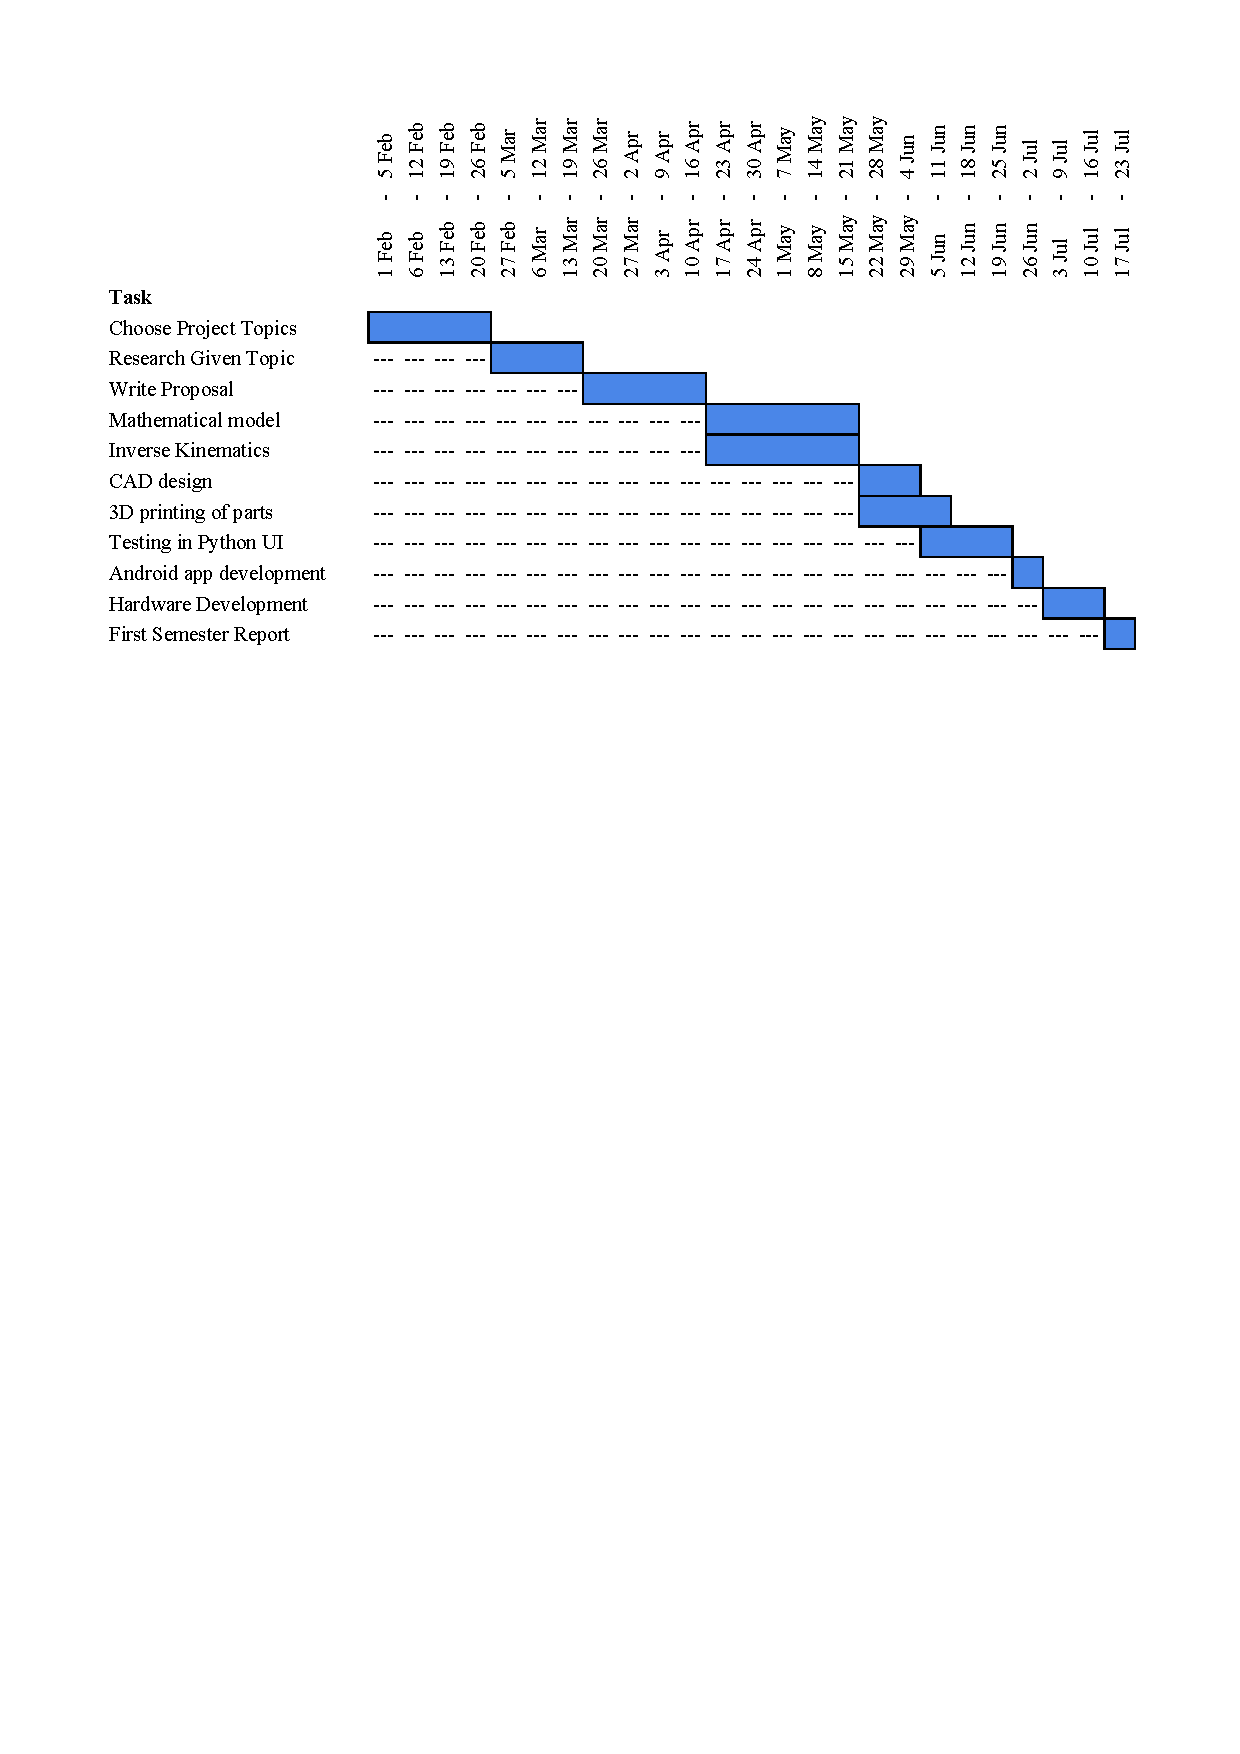
\includegraphics[clip, trim=1.5cm 18cm 1.5cm 1.5cm, width=1.00\textwidth]{pics/Gantt1.pdf}
    \caption{Gantt diagram for work already completed}
    \label{fig:Gantt1}
\end{figure}

Figure \ref{fig:Gantt2} below shows the remaining time in the project period. The blocks coloured in purple therefore represent work that still has to be completed.

\FloatBarrier
\begin{figure}[H]
    \centering
        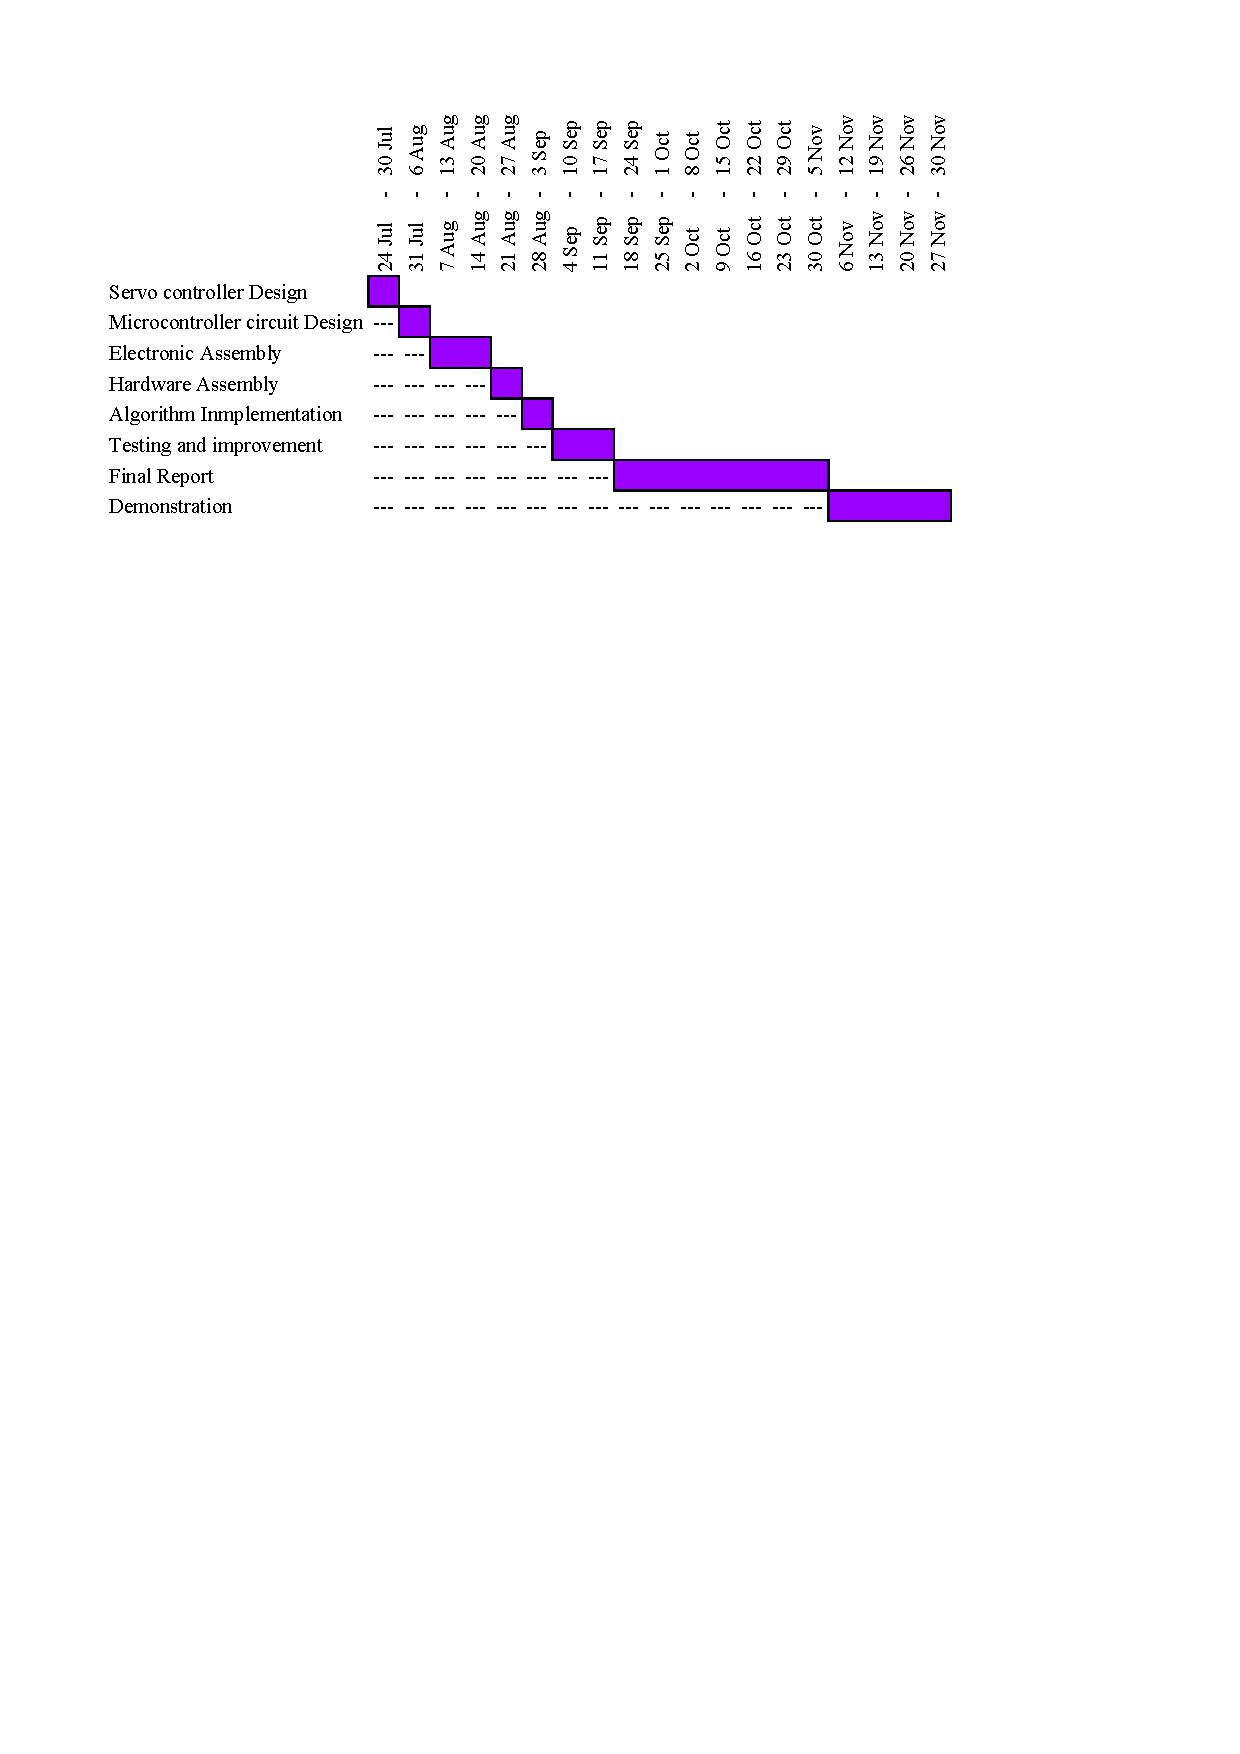
\includegraphics[clip, trim=1.5cm 21cm 1.5cm 1.5cm, width=1.00\textwidth]{pics/Gantt2.pdf}
    \caption{Gantt diagram for work to be completed}
    \label{fig:Gantt2}
\end{figure}
\FloatBarrier

%\vspace{30cm}

%\newpage

%% End of File.


%%
%%  Department of Electrical, Electronic and Computer Engineering.
%%  EPR400/2 Project Proposal - Section 4.
%%  Copyright (C) 2011-2017 University of Pretoria.
%%

\section{Specifications}

\subsection{Mission-critical system specifications}

\begin{center}
\begin{longtable}{|p{5cm}|p{5cm}|p{5cm}|}
\hline
  \textbf{SPECIFICATION (IN MEASURABLE TERMS)} &
  \textbf{ORIGIN OR MOTIVATION OF THIS SPECIFICATION} &
  \textbf{HOW WILL YOU CONFIRM THAT YOUR SYSTEM COMPLIES WITH
           THIS SPECIFICATION?}\\
\hline
   &
   &
   \\
\hline
   &
   &
   \\
\hline
   &
   &
   \\
\hline
\caption{Mission-critical system specification}
\end{longtable}
\end{center}

\subsection{Field conditions}

\begin{center}
\begin{longtable}{|p{7.5cm}|p{7.5cm}|}
\hline
  \textbf{REQUIREMENT} &
  \textbf{SPECIFICATION (IN MEASURABLE TERMS)} \\
\hline
   &
   \\
\hline
   &
   \\
\hline
   &
   \\
\hline
\caption{Field conditions}
\end{longtable}
\end{center}

\subsection{Functional unit specifications}

\begin{center}
\begin{longtable}{|p{7.5cm}|p{7.5cm}|}
\hline
  \textbf{SPECIFICATION} & \textbf{ORIGIN OR MOTIVATION} \\
\hline
   &
   \\
\hline
   &
   \\
\hline
\caption{Functional unit specifications}
\end{longtable}
\end{center}

\newpage

%% End of File.



%%
%%  Department of Electrical, Electronic and Computer Engineering.
%%  EPR400/2 Project Proposal - Section 5.
%%  Copyright (C) 2011-2017 University of Pretoria.
%%

\section*{5. Deliverables}
\addcontentsline{toc}{subsection}{5. Deliverables}

\subsection*{Technical deliverables}

\begin{center}
\begin{longtable}{|p{7cm}|p{3.5cm}|p{3.5cm}|}
\hline
\textbf{DELIVERABLE} & \textbf{DESIGNED AND IMPLEMENTED BY STUDENT} &
\textbf{OFF-THE-SHELF} \\
\hline  Microcontroller for control of the robot.
         &     & \multicolumn{1}{c|}{X}\\
\hline Control code for inverse kinematics and servo control.
         &   \multicolumn{1}{c|}{X}  &  \\
\hline Android application with a user interface for control of the robot.
         &   \multicolumn{1}{c|}{X}  &  \\
\hline Wireless module for communication between the smartphone interface and the robot
         &     &  \multicolumn{1}{c|}{X}\\
\hline Circuits implemented on PCB for interfacing all hardware with the microcontroller.
         &  \multicolumn{1}{c|}{X}   &  \\
\hline Servo motors for movement of the joints.
	&	&\multicolumn{1}{c|}{X}	\\
	\hline Robot body and legs.
	&	\multicolumn{1}{c|}{X}&	\\
	\hline Simulations on all implemented software and analogue design
	&	\multicolumn{1}{c|}{X}&	\\
\hline
\caption{Deliverables}
\end{longtable}
\end{center}

\subsection*{Demonstration at the examination}
\begin{enumerate}
\item The robot will be placed on a grid on the floor and the examiners will be shown that the robot is capable of holonomic movement.
\item The centre of the robot will be noted on the grid and the examiners will see that the robot is capable of rotating around its centre without translating.
\item The robot will execute a specific set of movements while the time to completion is being recorded.
\item Small obstacles will be placed in the way of the robot to make movement more challenging. This includes small blocks to step over as well as a change in surface such as sand.
\item The robot will repeat the set of movements over the obstacles while the time to completion is measured again.
\item The examiners will see that the robot is capable of moving with similar effort over various surfaces.
\end{enumerate}

\newpage

%% End of File.



\setcounter{subsection}{5}
\titleformat{\subsection}[frame]
{\fontsize{12pt}{14.4pt}\selectfont\bfseries} {} {5pt} {\thesubsection\quad}
\printbibliography[heading=subbibnumbered]
\end{refsection}
%Main report
%\newpage
\setcounter{subsection}{0}
%Change formatting for tis section

\titleformat{\section}[frame]
{\fontsize{24pt}{28.8pt}\selectfont\bfseries} {} {5pt} {}
\titleformat{\subsection}[display]
{\fontsize{18pt}{21.6pt}\selectfont\bfseries} {} {5pt} {\thesubsection\quad}
\titleformat{\subsubsection}[display]
{\fontsize{14pt}{16.8pt}\selectfont\bfseries} {} {5pt} {\thesubsubsection\quad}
\renewcommand\thesubsection{\arabic{subsection}.}
\renewcommand\thesubsubsection{\arabic{subsection}.\arabic{subsubsection}}
\rhead{\rightmark}

%Start
\section*{Part 4. Main report}
\addcontentsline{toc}{section}{Part 4. Main report}
\markright{Part 4. Main report}
\secun{Literature study}
\pagenumbering{arabic}
\subsubsection{Background and context}

\subsubsection{Application of background to this project}
In this section of the report, a brief overview of the existing research that is relevant to this project will be given, as well as a short discussion on how this existing research will be used to aid in the design of a five legged holonomic robot during the course of this project.\\

Legged vehicles are preferred to wheeled vehicles for exploration and rescue in remote areas because of their ability to cross rough terrain quickly with a severely reduced risk of getting stuck. The price to pay for this superior drive-train is far more complex electronics and movement algorithms \cite{Hidayat:Autonomous}. Instead of just driving the wheel motors and steering, each limb actuator of each leg has to be controlled to move to a calculated position.\\ 

Inverse kinematics is the mathematical process used to calculate the required angles of the limbs of a structure to reach a specific set of coordinates. This is used extensively in this project because of its ability to easily transform desired Cartesian coordinates into the required actuator angles. In the paper \cite{Oh:Analytic}, a method is discussed for solving the inverse kinematic equations involved in a seven degrees of freedom robotic arm. This method takes into account specified minimum and maximum values for each actuator and degree of freedom in order to avoid self-collision. This method can be applied to any system with a specified degrees of freedom and can therefore be simplified to solve the inverse kinematic equations for the system designed in this project.\\

To obtain the Cartesian coordinates desired at any given time, the method described in \cite{Hidayat:Autonomous}, namely Sine pattern methods is used. In \cite{Hidayat:Autonomous}, the method was applied to a quadruped robot. In the case of this project, the method is expanded to make it suitable for use on a robot with five legs. Adaptation is required because the method relies on the symmetry of a quadruped robot to schedule the lifting of the legs. Since the same symmetry does not exist in a robot with five legs, a different scheduling technique is investigated. This method will rely on information from the current position of the legs, the limits of leg movement, as well as the current horizontal tilt of the robot.\\

In the conference paper \cite{Jain:Odometry}, motion planning of omnidirectional robots is discussed and a sophisticated yet simple and efficient method of route planning is proposed. This method is based on vehicles that use three omnidirectional wheels in combination to form a resultant force vector in the desired direction. These type of vehicles differ largely in terms of locomotion when compared to the holonomic legged design used in this project, but there are a few key similarities. Both these designs can move holonomically, therefore they have the ability to move in a straight line while rotating, move in an arc without rotating, or any combination of the two. These similarities mean that some of the methods discussed and applied in \cite{Jain:Odometry} can be used to aid in the design of the algorithm used in this project.\\

A team from Instituto Tecnologico de la Laguna in Mexico designed a hexapod robot \cite{Ollervides:Navigation} similar to the robot designed in this project. The purpose of the hexapod was to investigate its potential for use in exploration of areas that are hard to reach by any commonly used means of transportation. Legged vehicles are more suited to cross rough terrain, but rough terrain complicates the design of the drive-train. In applications where the surface is smooth or close to smooth, open loop control can be applied where the leg is simply moved to the desired position and it is assumed by the designer that the robot foot is making contact with the ground at this point, and therefore supporting part of the distributed robot weight. When the robot is crossing rough terrain, where the surface consists of mainly bumps and holes, this assumption could be false. In such a scenario, the robot could lift another leg while under the impression that its weight is being supported by the other legs. If this is not the case, the robot could fall over and possibly damage itself or be unable to rectify itself. To avoid this problem, closed loop control should be used in the height positioning of the legs. This involves having a sensor in the system that could provide feedback on the state of the foot. The hexapod in \cite{Ollervides:Navigation} used miniature resistive force sensors attached to the bottom of each foot of the robot. The robot therefore has the ability to take analogue measurements from these sensors and determine the weight distribution of the individual feet of the robot. This data is used to confirm that all robot feet are making contact with the surface and correct the situation if this is not the case. This type of feedback is also useful when the robot is operated on slanted surfaces because of the effect that the center of gravity has on a slanted surface. A feedback sensor will be included in the design of the five legged holonomic robot in this project.\\

If the robot is operating on a slanted surface without it being aware of this and the centre of gravity shifts over the lowest foot making contact, the robot could fall over even when all of its legs are making contact with the surface. In a paper on reactive robot navigation \cite{Arkin:Reactive}, it is proposed that the use of a digital inclinometer can aid in solving this problem. The sensor provides information on the current tilt of the robot in two dimensions. This sensor in combination with the feedback sensors on the robot feet can be used to ensure that the robot levels itself automatically to avoid tipping over. The data collected from this sensor can also be used to collect information on the terrain. In the journal article \cite{Arkin:Reactive}, this data is used for hill climbing as well as finding valleys in unexplored areas. In order to enable the robot designed in this project to walk on slanted surfaces, a digital inclinometer will be used. Some of the reactive navigation techniques discussed in \cite{Arkin:Reactive} will also be implemented to aid the robot in navigating on slanted planes.\\

In a paper on the effects of slippery surfaces on biped robots \cite{Hyeon:Reflex}, methods on avoiding falling over of a biped robot is investigated. Since these robots have to balance themselves to stay upright, an unforeseen slippery patch on a surface could be fatal for the robot. If it were possible to foresee a slippery surface, slowing down the walking gait and increasing foot surface would help increase the traction of the robot, and therefore lower the risk of slipping. Since a five legged robot is inherently stable and there is no balancing required, slippery surfaces may influence the traction of the robot but there is very low risk of falling over on level surfaces that are slippery. It is therefore suitable to just slow down movements on slippery surfaces to increase the traction where possible.

\secun{Approach}
This section outlines the initial approach to solve the functions shown in the functional block diagram. The functional block diagram of the project can be found in Figure \ref{fig:Func}
\subsubsection{Design alternatives}

\subsubsection{Preferred solution}



\secun{Design and implementation}
\subsubsection{Background}
A large part of the design of a legged robot depends on the design of a simple leg - more specifically the degrees of freedom that a single leg has. The degrees of freedom that a single leg has is determined by the amount of dimensions that the leg can make a controlled movement in, independently from any other dimensions. There are two common underlying designs in robot leg design - these are for two and three degrees of freedom respectively.\\

Figure \ref{fig:2DOF} shows an example of a common design that has two degrees of freedom. The design therefore contains two joints in one leg. In this example, the first joint is positioned vertically to form the hip op the robot leg. This allows for the side-to-side motion required for walking. The second joint is positioned horizontally to allow the lowest limb to move up and down. The two degrees of freedom controlled by this leg design is therefore the horizontal angle of the leg and the height of the foot. These two (and only these two) parameters can therefore be controlled completely independently.
\FloatBarrier
\begin{figure}[h]
\centering
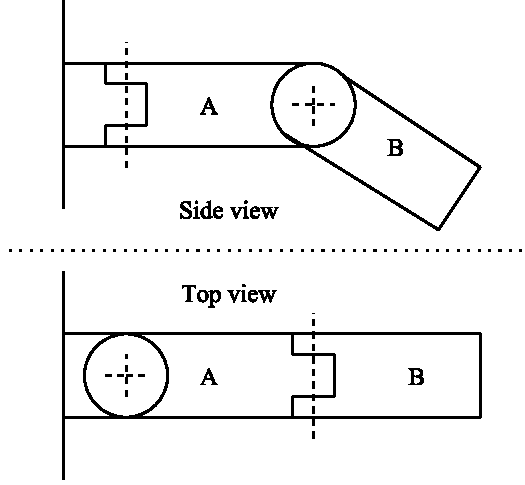
\includegraphics[scale = 1]{pics/2DOF.pdf}
\caption{Example of a leg design with two degrees of freedom.}
\label{fig:2DOF}
\end{figure}
\FloatBarrier
An example of a robotic leg with three degrees of freedom can be seen in Figure \ref{fig:3DOF}. This design is similar to that of the leg with two degrees of freedom seen in Figure \ref{fig:2DOF}, with the only addition being a second horizontal joint further down from the first. This additional limb means that the horizontal distance from the foot to the hip can be controlled as well as the height of the foot. These two controlled parameters, together with the horizontal leg angle which can also be controlled independently as in the case of the two degrees of freedom design, means that this design has a total of three degrees of freedom.
\FloatBarrier
\begin{figure}[h]
\centering
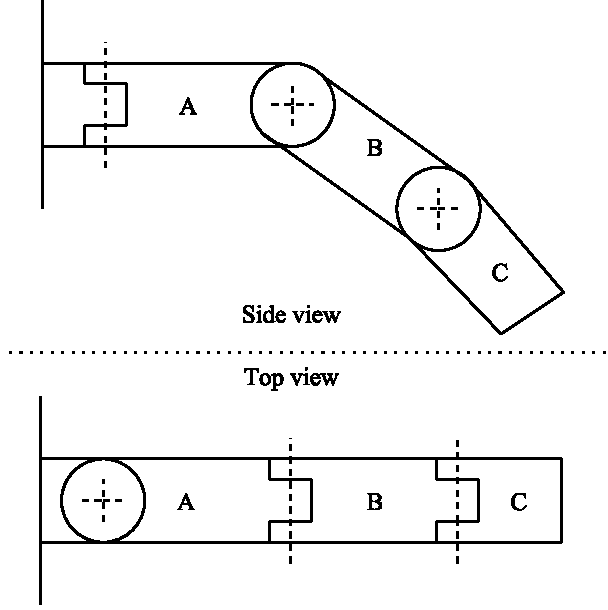
\includegraphics[scale = 1]{pics/3DOF.pdf}
\caption{Example of a leg design with three degrees of freedom.}
\label{fig:3DOF}
\end{figure}
\FloatBarrier


The design with three degrees of freedom has the advantage of being able to lift a leg without altering the horizontal position of the leg. This means that the robot is able to walk without altering the height of the body of the robot. The robot is therefore able to cross rougher terrain much better because of the ability to alter the height of the robot feet as the terrain requires. With the design that has two degrees of freedom, the foot height is a function of the horizontal extension of the leg. With this design the main advantage is the simplicity - both mechanically and in software. The cost and power consumption will also be much lower because of the reduced amount of actuators.\\

Due to the much greater flexibility of the design with three degrees of freedom and the ability to cross rougher terrain, this will be the platform implemented in the final design.\\

\subsubsection{Theoretical analysis and modelling}
\FloatBarrier
\begin{figure}[h]
\centering
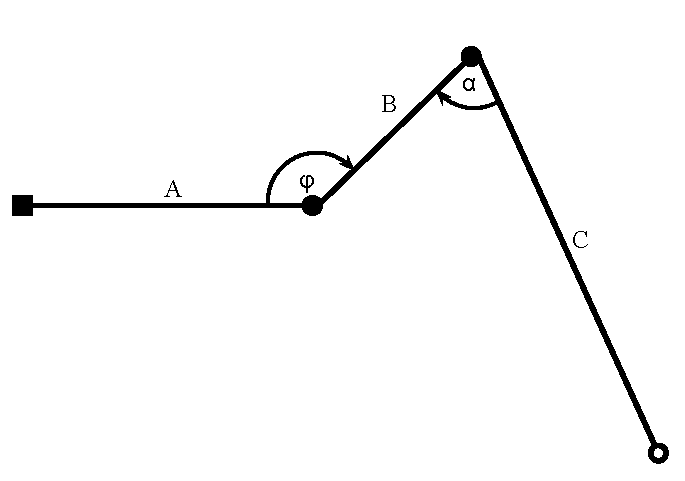
\includegraphics[scale = 1]{pics/Leg_design.pdf}
\caption{Simulation results for the network.}
\label{fig:Leg_design}
\end{figure}
\FloatBarrier

\FloatBarrier
\begin{figure}[h]
\centering
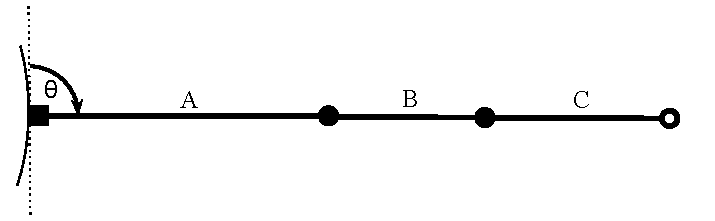
\includegraphics[scale = 1]{pics/Leg_design_2.pdf}
\caption{Simulation results for the network.}
\label{fig:Leg_design}
\end{figure}
\FloatBarrier

\subsubsection{Simulation}
\label{sec:sim}
In order to test the equations and design outlined in the Theory section above, the mathematics was implemented in a script written in the Python programming language and developed in the PyCharm IDE. The program consists of a GUI  used to enter elementary commands, similar to that implemented in the Android application, as well as a window for plotting the result in a 3-dimensional Cartesian system. Some results showing the validity of the design equations in the previous section can be found below. All of the source code used to build this simulation can be found in Part 5 of this report on the attached optical disc.\\

The program flow of the software in the simulation is similar to that used for the final prototype software, more information on the software design flow can be found in Section \ref{sec:soft}. The main difference between the final implementation and the simulation is that once the angle values for theta, alpha and phi are calculated for each leg, in the final implementation the result is used to move the actuator while in simulation the result is used to calculate the Cartesian position of each limb in order to plot it in the 3-dimensional system. It should be noted that the length of all of the limbs as well as the robot body radius was chosen as unity for simplicity and since the purpose of the simulation is only to show the functionality of the IK. It should also be noted that although some of the legs may look crooked in the following figures, this is only a result of the viewing angle. When viewed directly from above, all limbs of a single leg align in an upright plane.\\

The basic user interface together with the Robot in its neutral position can be seen in Figure \ref{fig:Sim1}.\\

The orange markers found at each of the robot feet indicate the neutral position for each of the five feet. This is indicated to aid in showing the movement of the legs relative to this neutral position in Figure \ref{fig:Sim1} and the figures following in this section.\\

\begin{figure}[H]
\centering
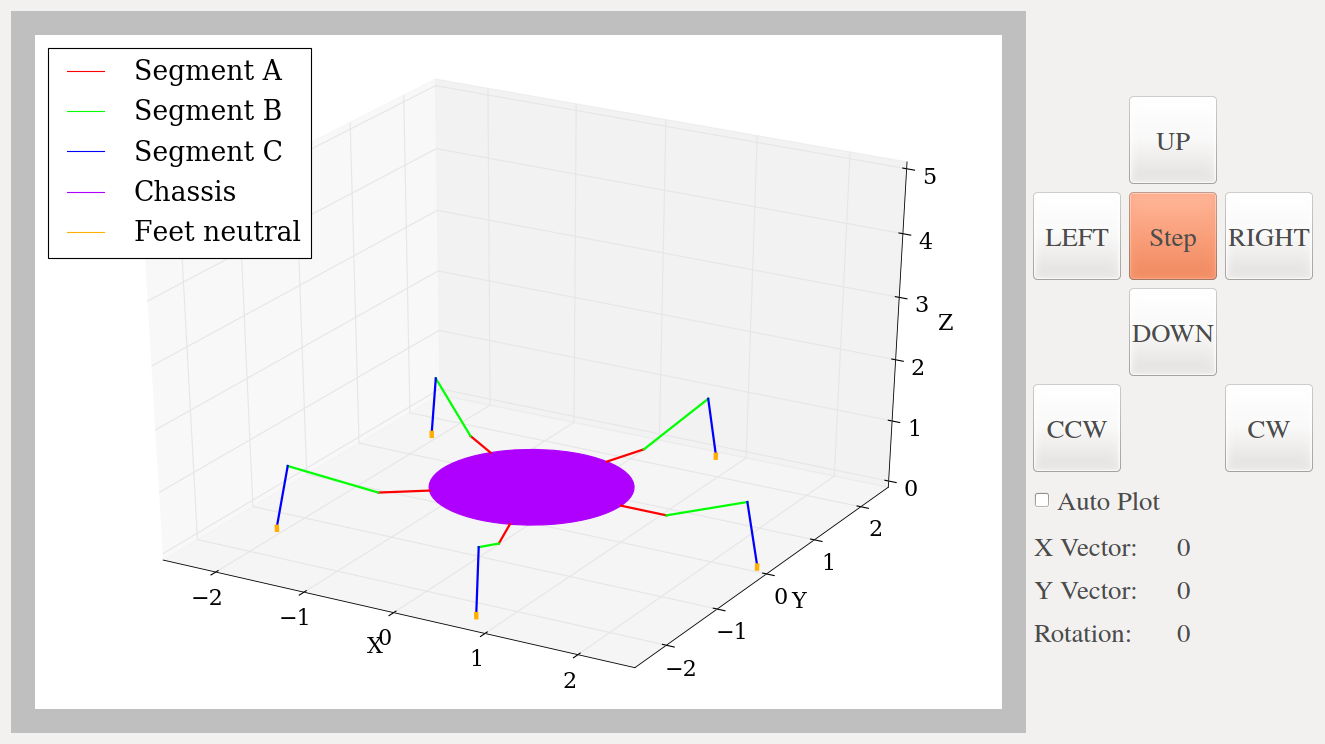
\includegraphics[scale = 0.33]{pics/Sim1.png}
\caption{Simulation window showing the robot in its neutral position.}
\label{fig:Sim1}
\end{figure}

When the $Y$ vector is changed to a positive value, the legs will all move in a negative $Y$-direction since the robot center is the origin. When the robot should move in a specific direction, the feet will move in the exact opposite direction to propel the robot forward. This is illustrated in Figure \ref{fig:Sim2}.

\begin{figure}[H]
\centering
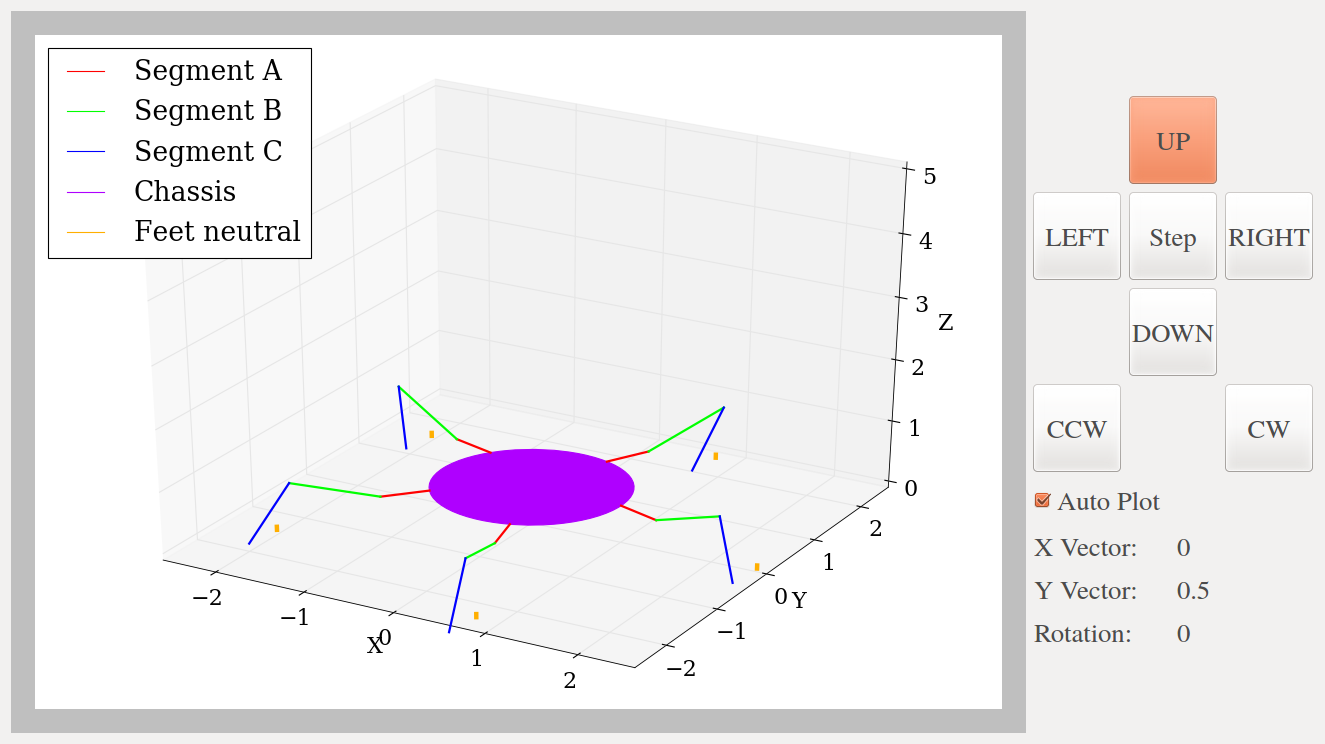
\includegraphics[scale = 0.33]{pics/Sim2.png}
\caption{Simulation window showing the robot moving in a positive $Y$-direction.}
\label{fig:Sim2}
\end{figure}

The robot should also be able to translate in the $X$-direction without making a rotation first. This is illustrated in Figure \ref{fig:Sim3}.

\begin{figure}[H]
\centering
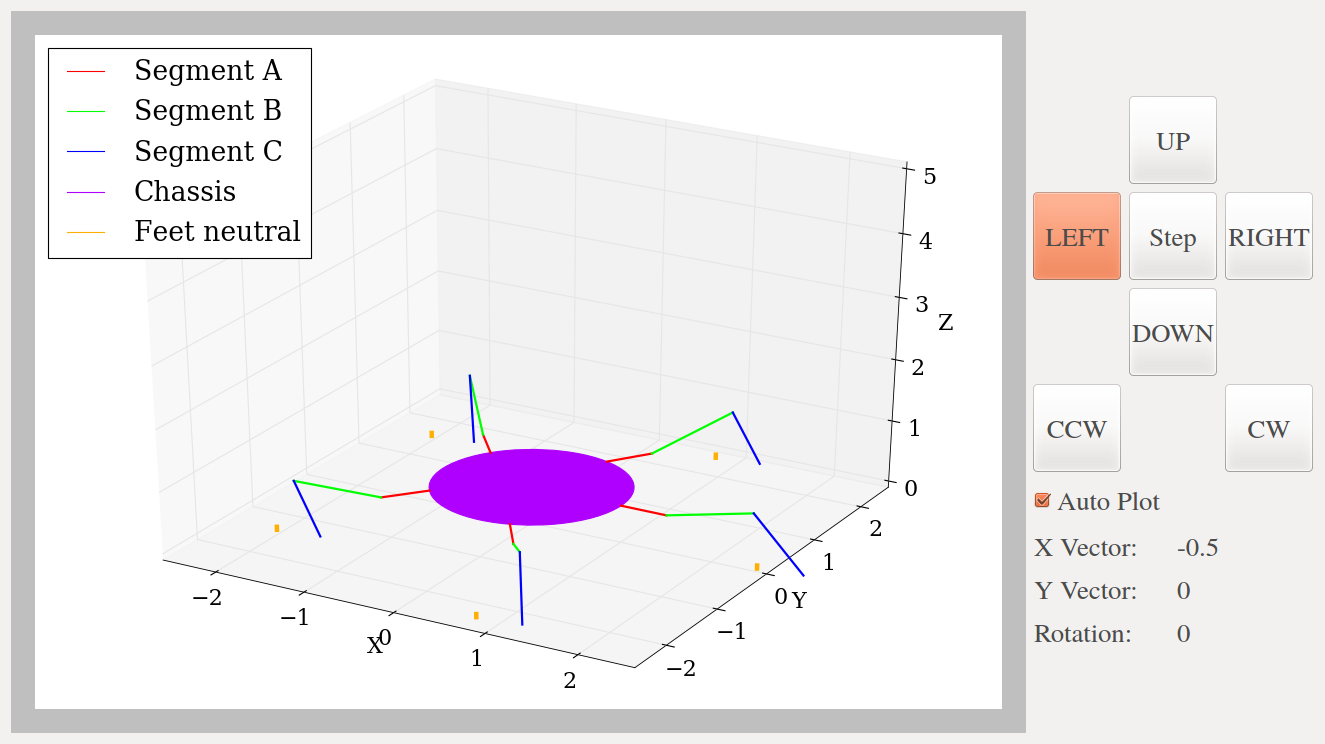
\includegraphics[scale = 0.33]{pics/Sim3.png}
\caption{Simulation window showing the robot moving in a negative $X$-direction.}
\label{fig:Sim3}
\end{figure}

If the robot can instantaneously move in both the $X$ and $Y$-directions, it should be able to move in a combination of the two without a problem. This ability is illustrated in Figure \ref{fig:Sim4}.

\begin{figure}[H]
\centering
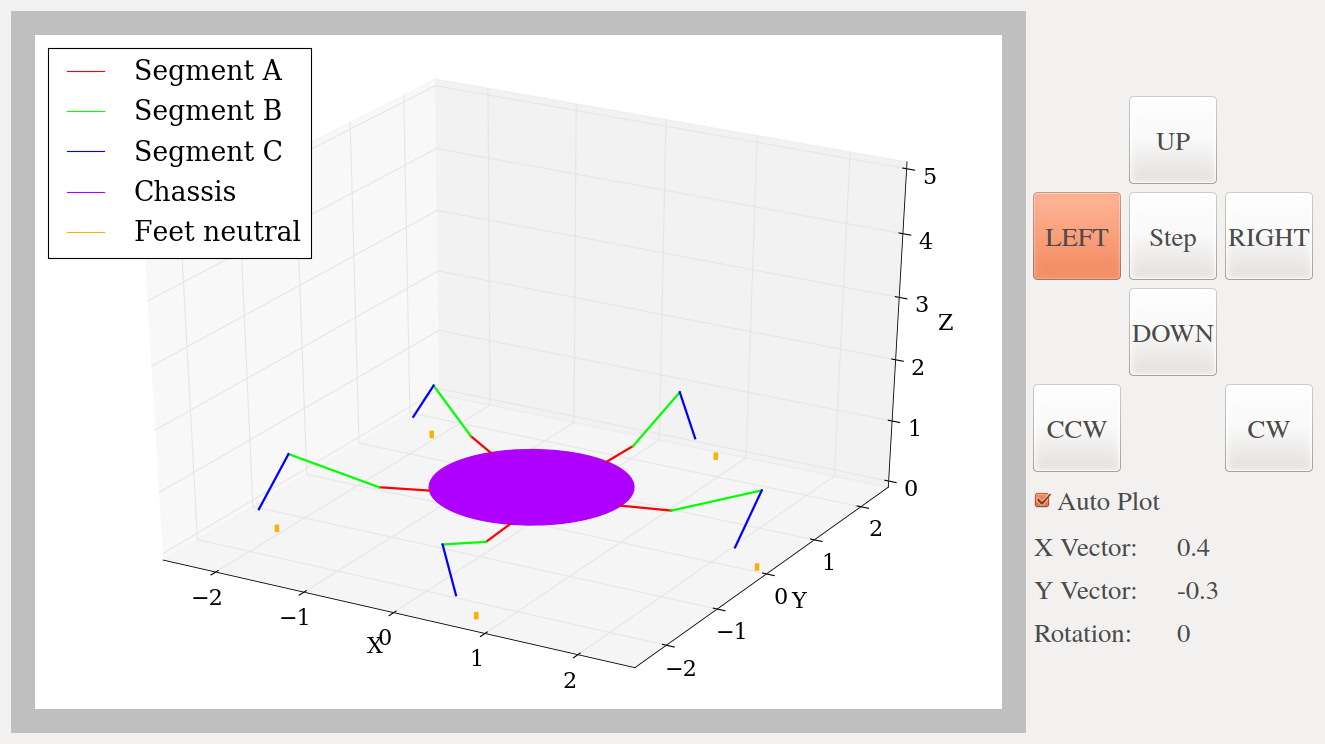
\includegraphics[scale = 0.33]{pics/Sim4.png}
\caption{Simulation window showing the robot moving in a direction with a positive $X$ and negative $Y$-component.}
\label{fig:Sim4}
\end{figure}

The translation appears to be working exactly as intended and designed for. The simulation is tested with a clockwise direction rotation in Figure \ref{fig:Sim5}.

\begin{figure}[H]
\centering
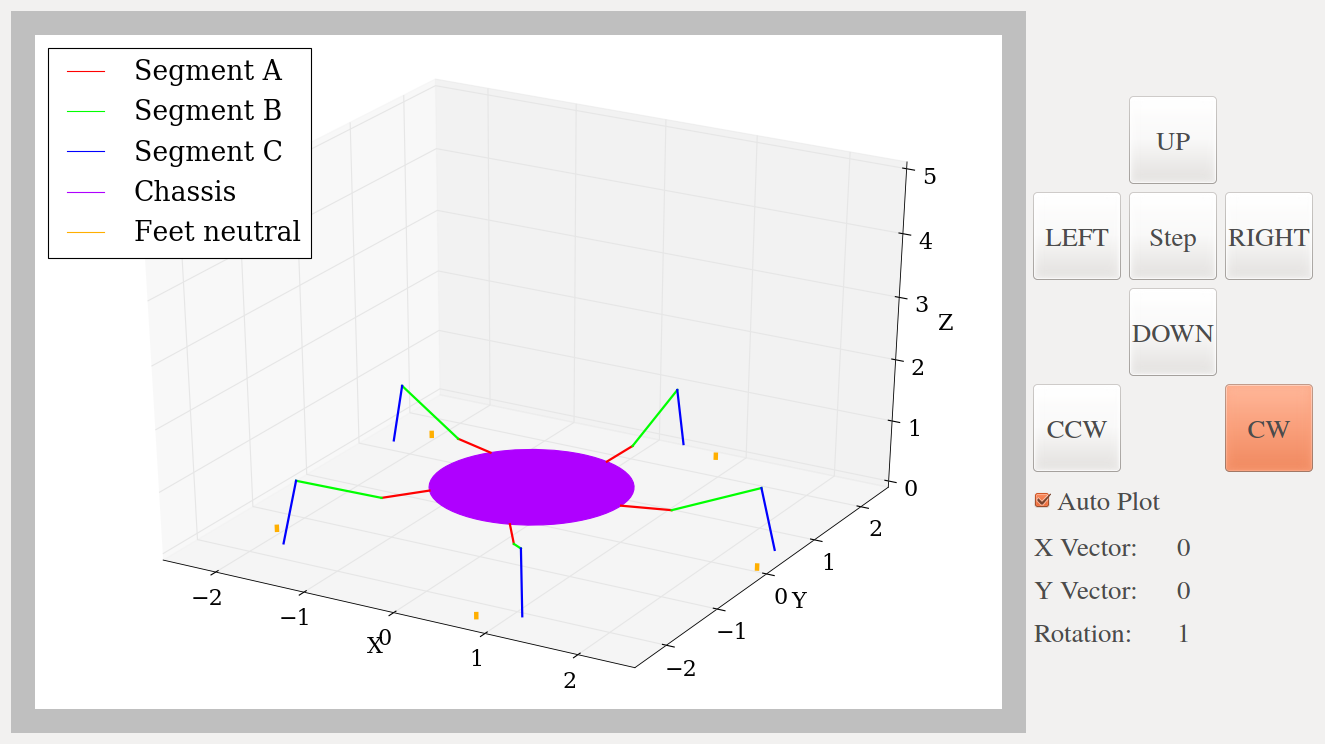
\includegraphics[scale = 0.33]{pics/Sim5.png}
\caption{Simulation window showing the robot rotating in a clockwise direction.}
\label{fig:Sim5}
\end{figure}

Once the robot reaches the boundary illustrated in Figure \ref{fig:Body_layout_3} for any of its legs, it is necessary to lift the leg up, move it to a more suitable location and put it down in order to continue in the direction it is heading in. This ability is illustrated in Figure \ref{fig:Sim6}.

\begin{figure}[H]
\centering
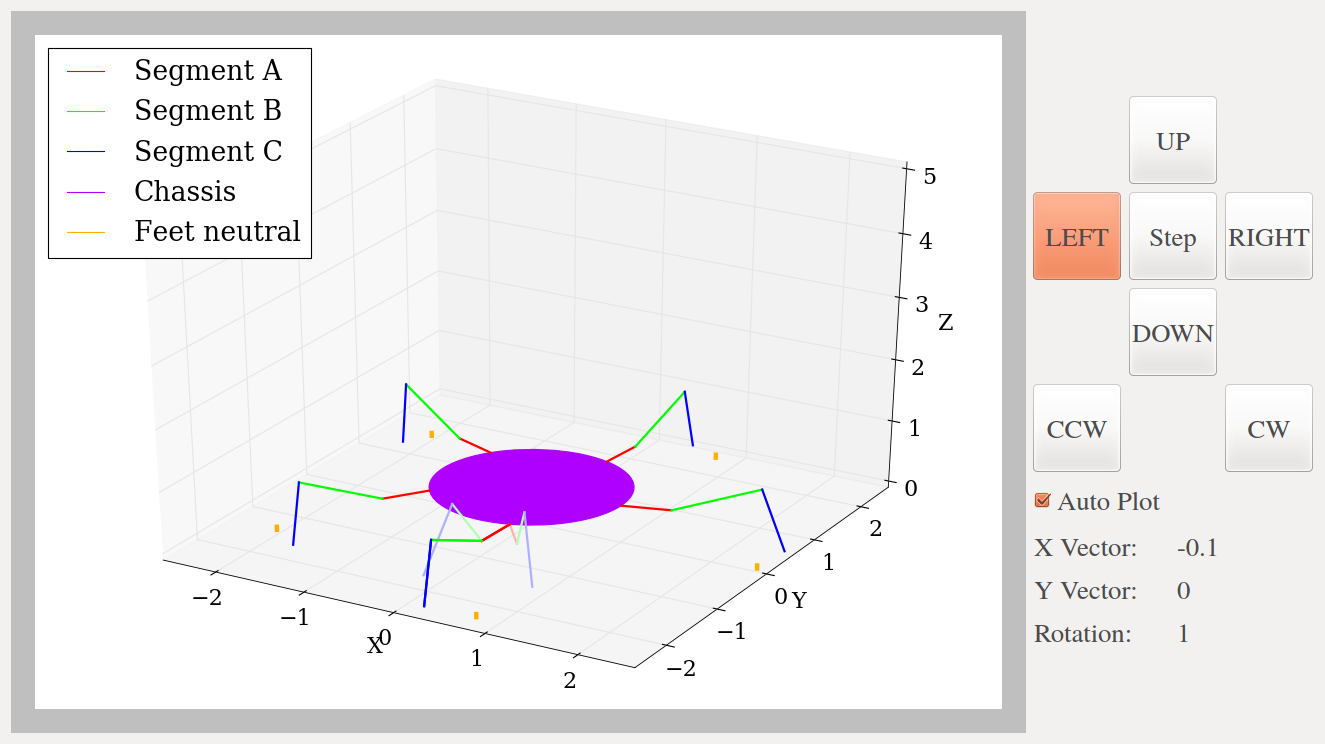
\includegraphics[scale = 0.33]{pics/Sim6.png}
\caption{Simulation window showing the robot picking up a foot and placing it again.}
\label{fig:Sim6}
\end{figure}

In Figure \ref{fig:Sim6}, the closest leg appears three times, twice in dimmed (ghost) colours and then finally in the normal colours. What this attempts to illustrate is the resetting motion of the leg. Figure \ref{fig:Sim5} shows the robot just before the resetting action. The right of the two "ghost" legs is right above the original location of the leg. This shows the position of the leg after it was lifted up. The left of the two "ghost" legs is the leg, still lifted, after being moved to a position directly over the new location. The leg plotted in full colour shows the final position of the leg. It is now able to start rotating further in the clockwise direction. Th robot will pickup and replace one leg at a time for all the legs that requires resetting and then continue.


\subsubsection{Optimisation}

\subsubsection{Hardware design}

\subsubsection{Hardware implementation}

\subsubsection{Software design}

\subsubsection{Software implementation}

\subsubsection{Design summary}


\secun{Results}

\subsubsection{Summary of results achieved}

\begin{tabular}{|p{5cm}|p{5cm}|p{5cm}|}
\hline
\textbf{Description of requirement or specification
(intended outcome)} & \textbf{Actual outcome}& \textbf{Location in report}\\
\hline
\multicolumn{3}{|l|}{}\\
\multicolumn{3}{|l|}{\textbf{Mission requirements of the product}}\\
\hline
1&2&3\\
\hline
\multicolumn{3}{|l|}{}\\
\multicolumn{3}{|l|}{\textbf{Field conditions}}\\
\hline
1&2&3\\
\hline
\multicolumn{3}{|l|}{}\\
\multicolumn{3}{|l|}{\textbf{Specifications}}\\
\hline
1&2&3\\
\hline
\multicolumn{3}{|l|}{}\\
\multicolumn{3}{|l|}{\textbf{Deliverables}}\\
\hline
1&2&3\\
\hline

\end{tabular}

\subsubsection{Qualification tests}
\titleformat{\section}[frame]
{\fontsize{24pt}{28.8pt}\selectfont\bfseries} {} {5pt} {}
\titleformat{\subsection}[display]
{\fontsize{18pt}{21.6pt}\selectfont\bfseries} {} {5pt} {\thesubsection\quad}
\titleformat{\subsubsection}[frame]
{\fontsize{14pt}{16.8pt}\selectfont\bfseries} {} {5pt} {\thesubsubsection\quad}
\renewcommand\thesubsection{\arabic{subsection}.}
\renewcommand\thesubsubsection{\arabic{subsection}.\arabic{subsubsection}}
\rhead{\rightmark}
%add paragraph as extra level for experiments
\setcounter{secnumdepth}{5}
\titleformat{\paragraph}[display]
{\fontsize{12pt}{14pt}\selectfont\bfseries}{}{5pt} {\theparagraph\quad}
%add subparagraph
\titleformat{\subparagraph}[display]
{\fontsize{12pt}{14pt}}{}{5pt} {\thesubparagraph\quad}
\renewcommand\thesubparagraph{\arabic{subsection}.\arabic{subsubsection}.\arabic{paragraph}\alph{subparagraph}}

\section*{Description of product}
\markright{Part 5. Technical documentation}

This report contains the technical documentation required to design a holonomic five legged robot. The robot is built using 15 servo motors, 3D printed parts, a 32 bit microcontroller and a smartphone application that functions as a user interface and remote control.
\newpage
\tableofcontents
\markright{Part 5. Technical documentation}
\newpage
\pagenumbering{arabic}
\setcounter {section}{1}


\secun{System block}

\begin{figure}[H]
\centering
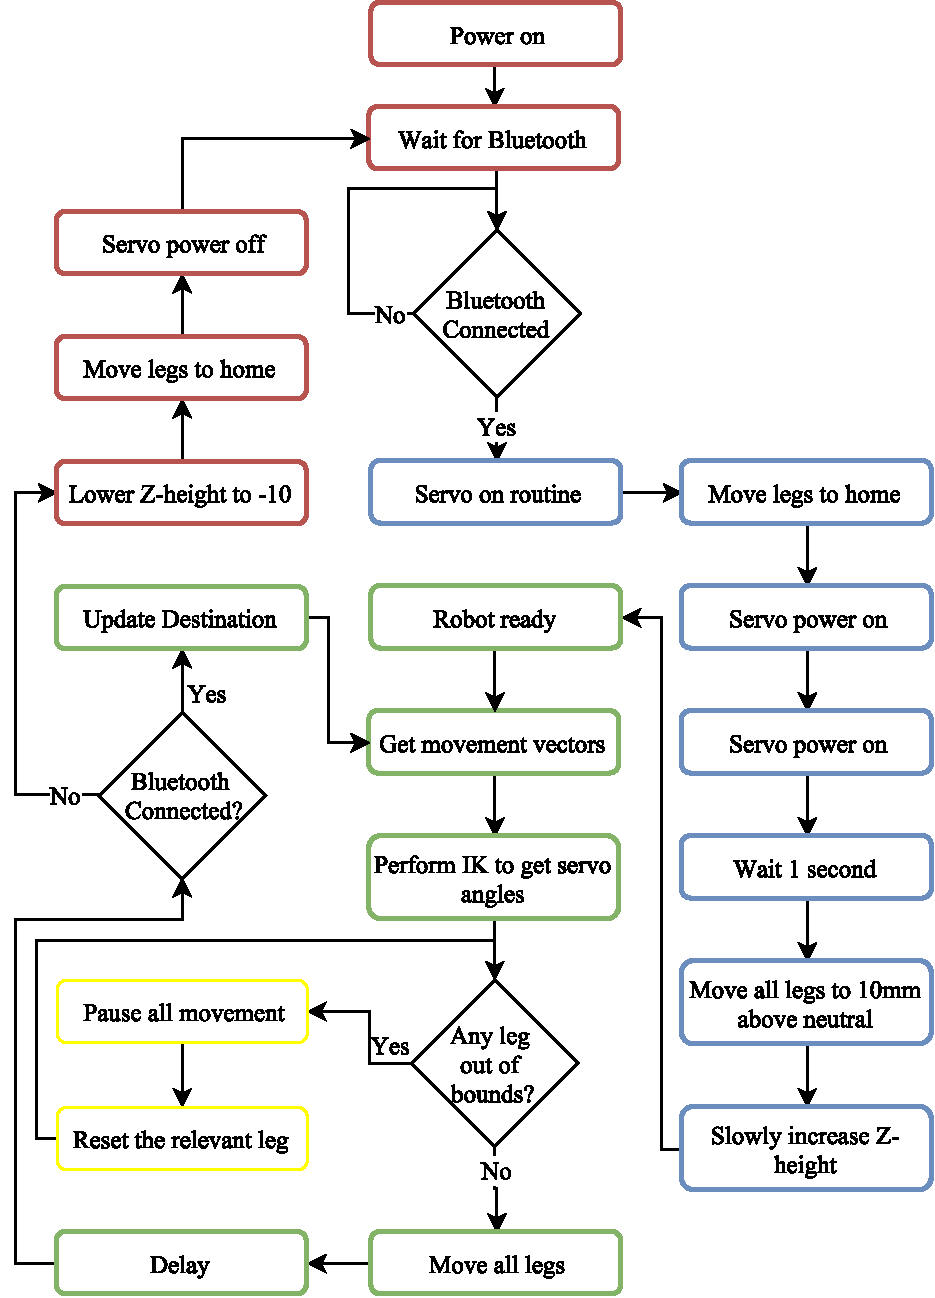
\includegraphics[scale = 0.8]{pics/Soft2.pdf}
\caption{System block diagram.}
\end{figure}

\secun{Systems level description of design}

\begin{figure}[H]
\centering
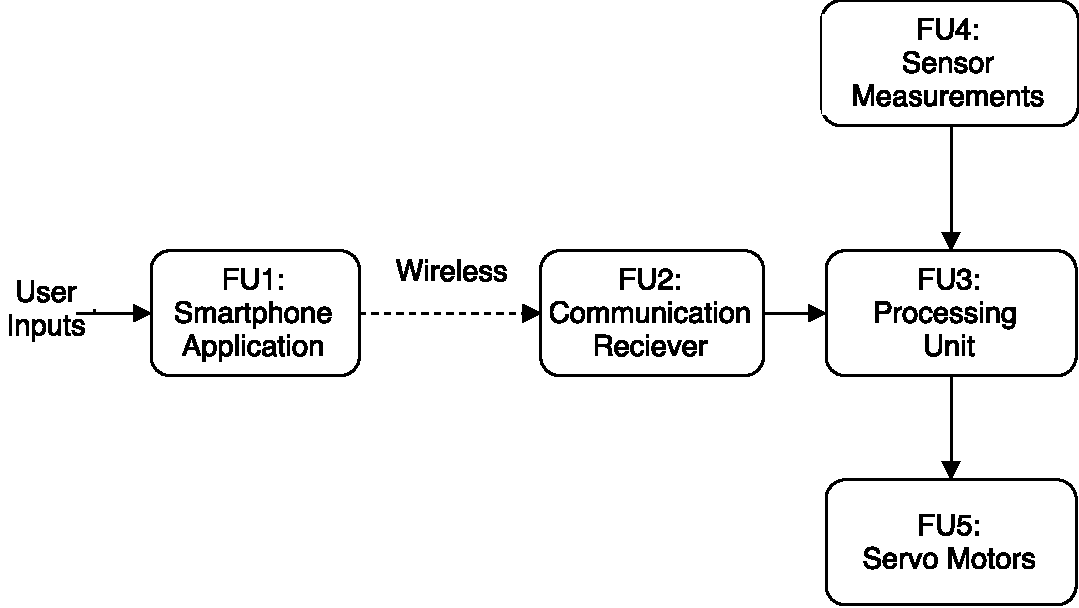
\includegraphics[scale = 0.5]{Proposal/FunctionalDiagram.pdf}
\caption{System level design.}
\end{figure}

\secun{Block diagrams of modules}
The design does not consist of modules. The system block diagram can be seen above\\
\secun{Description of modules}
The design does not consist of modules. The complete description of the design can be found in part 4 of this report.\\
\secun{Description of interfacing with other modules}
The only interfacing in this project is between the smartphone and the robot. More details on this can be found in part 4 of this report\\
\secun{Complete circuit diagram}
\begin{figure}[H]
\centering
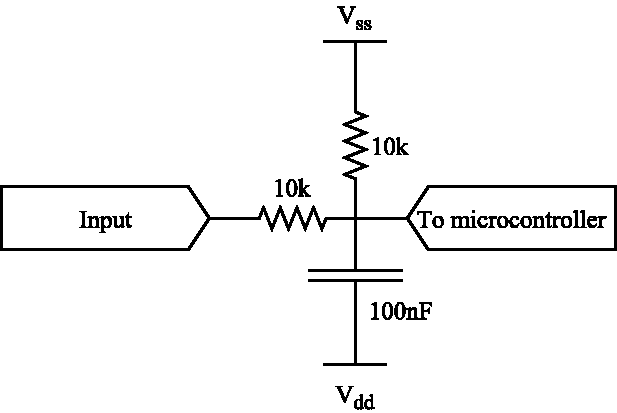
\includegraphics[scale = 1]{pics/InputProtection.pdf}
\caption{Input protection design.}
\end{figure}
\begin{figure}[H]
\centering
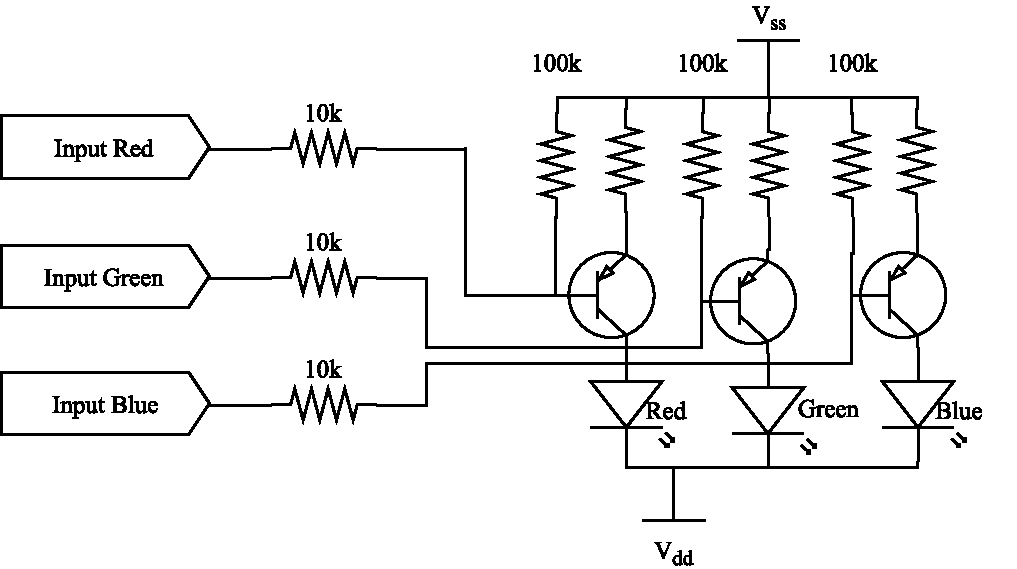
\includegraphics[scale = 1]{pics/LEDDriver.pdf}
\caption{LED driver design.}
\end{figure}
\begin{figure}[H]
\centering
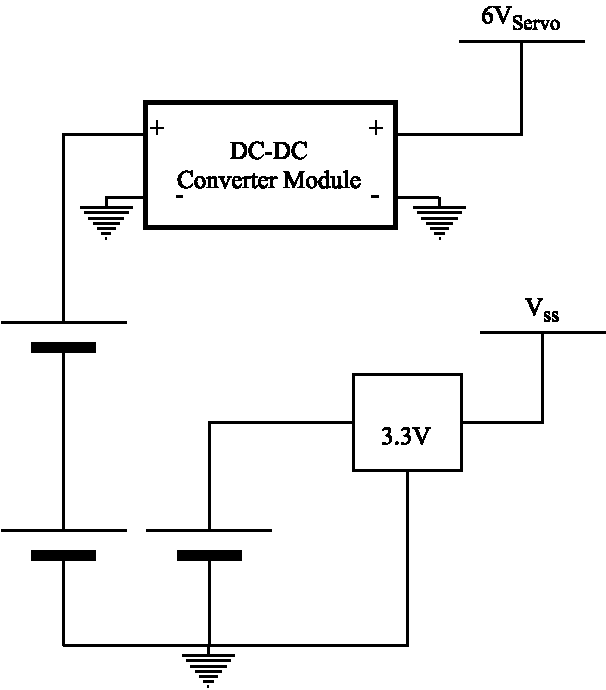
\includegraphics[scale = 1]{pics/PowerSupply.pdf}
\caption{Power supply design.}
\end{figure}
\begin{figure}[H]
\centering
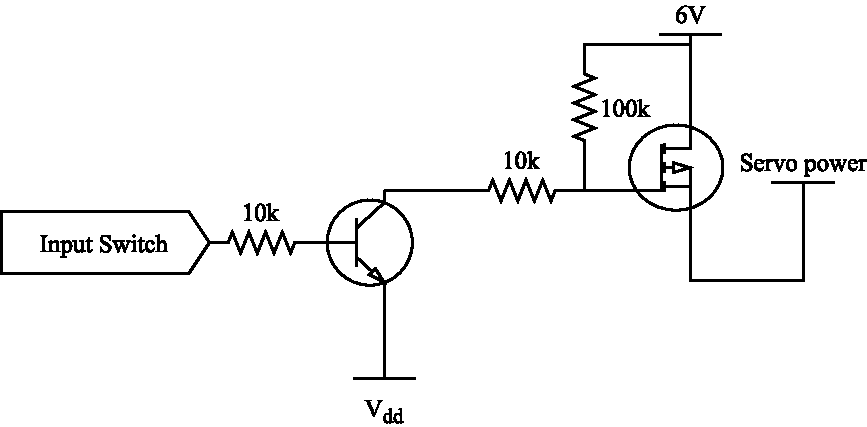
\includegraphics[scale = 1]{pics/PowerSwitch.pdf}
\caption{Power switch design.}
\end{figure}
\secun{Description of circuit}
All of the circuit diagrams displayed above is explained in detail in part 4 of this report\\

\secun{Circuit diagrams of modules}
The circuit diagrams for all modules are shown in record 6.\\

\secun{Description of circuit diagrams}
All of the circuit diagrams displayed above is explained in detail in part 4 of this report\\

\secun{Timing diagrams}
Timing diagrams is not applicable to this project.\\

\secun{VHDL code}
VHDL code is not applicable to this project.\\

\secun{PC board layout}
No PCB was designed for this project. The veroboard planning is outlined in record 13\\

\secun{Components placement on the board}
Since the central part of the robot electronics is the microcontroller used, it is placed in the centre of the Veroboard with the support electronics around it. The DC-DC converter was placed separately from the Veroboard.

\secun{Wiring diagram of the product mounted in the enclosure}
The product has no enclusure.\\

\secun{Mechanical design}
\begin{figure}[H]
\centering
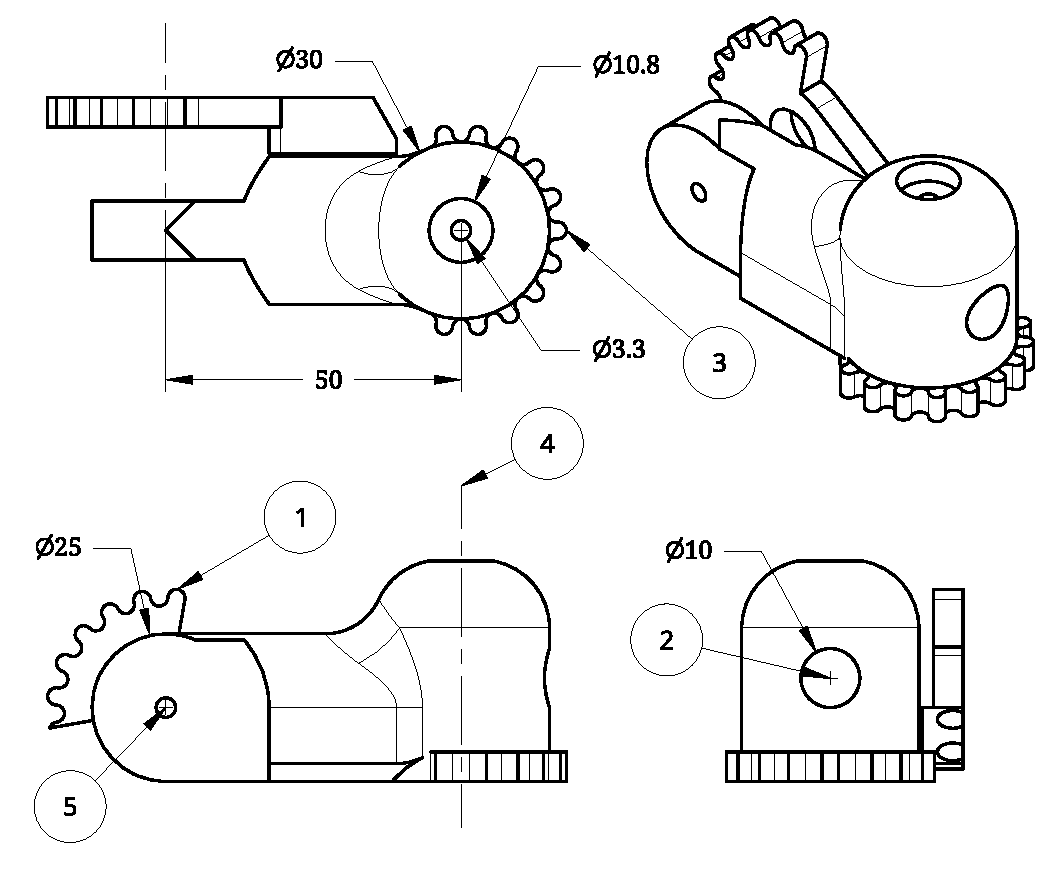
\includegraphics[scale = 1]{pics/DrawingA.pdf}
\caption{Leg A design.}
\end{figure}
\begin{figure}[H]
\centering
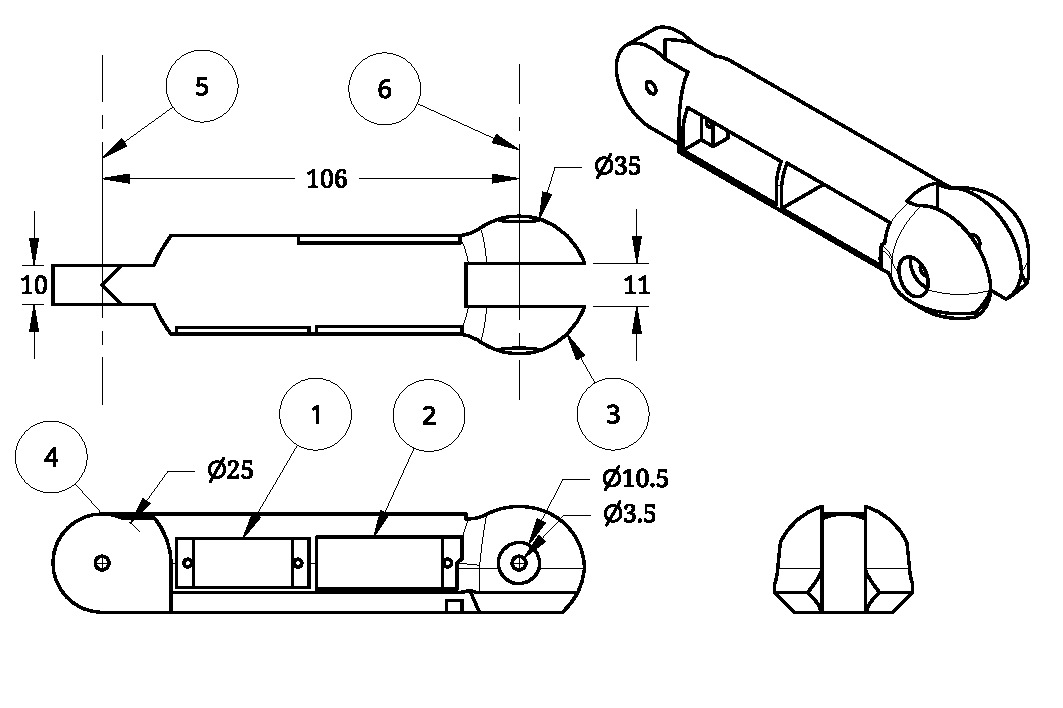
\includegraphics[scale = 1]{pics/DrawingB.pdf}
\caption{Leg B design.}
\end{figure}
\begin{figure}[H]
\centering
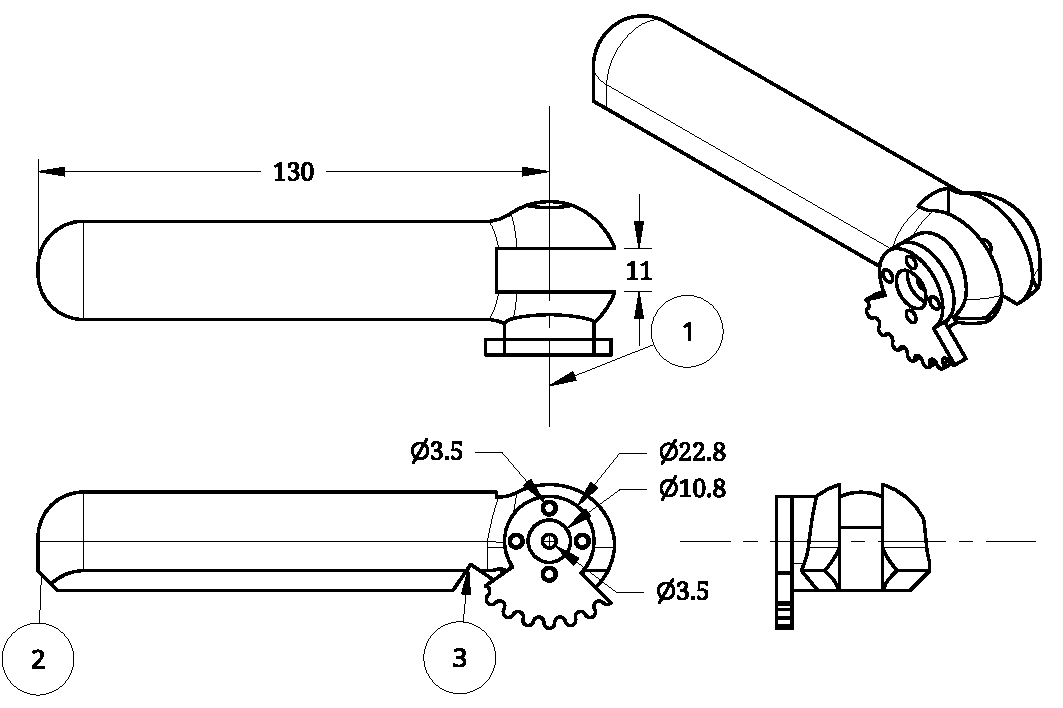
\includegraphics[scale = 1]{pics/DrawingC.pdf}
\caption{Leg C design.}
\end{figure}
\begin{figure}[H]
\centering
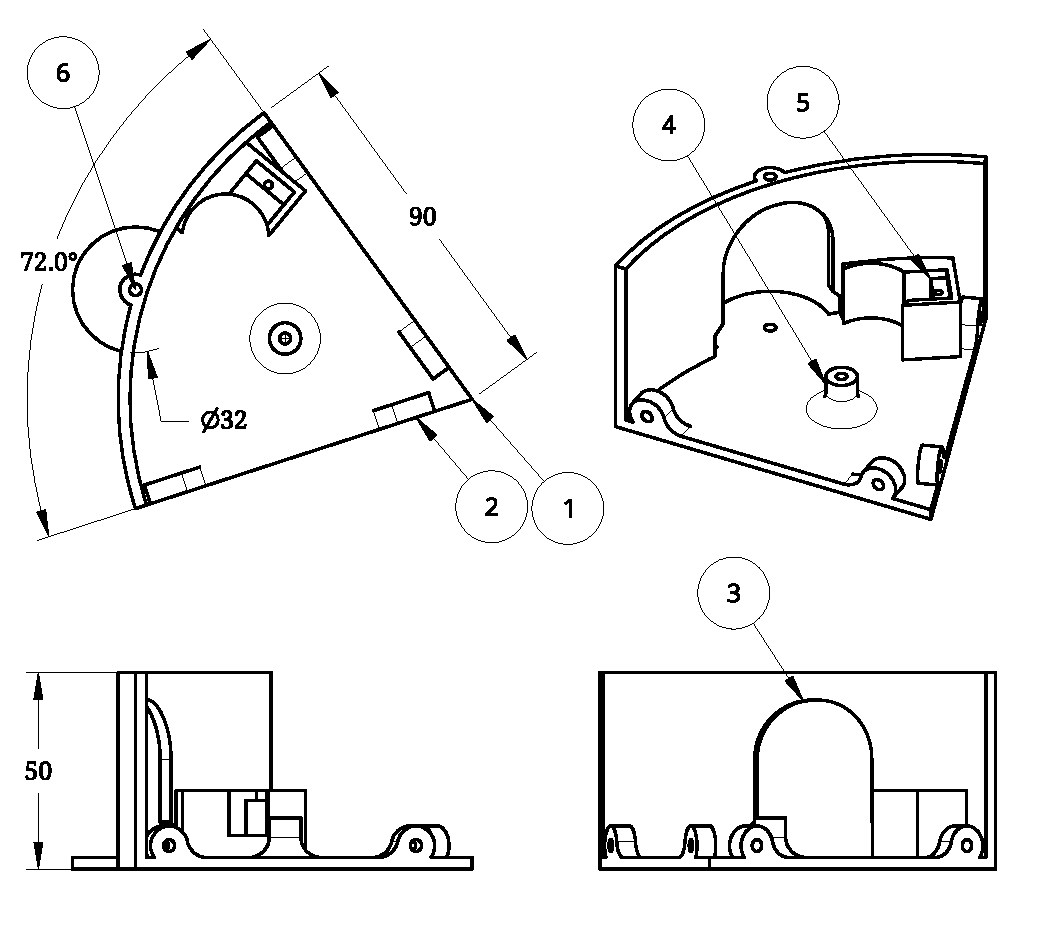
\includegraphics[scale = 1]{pics/DrawingBase.pdf}
\caption{Robot base design.}
\end{figure}
\begin{figure}[H]
\centering
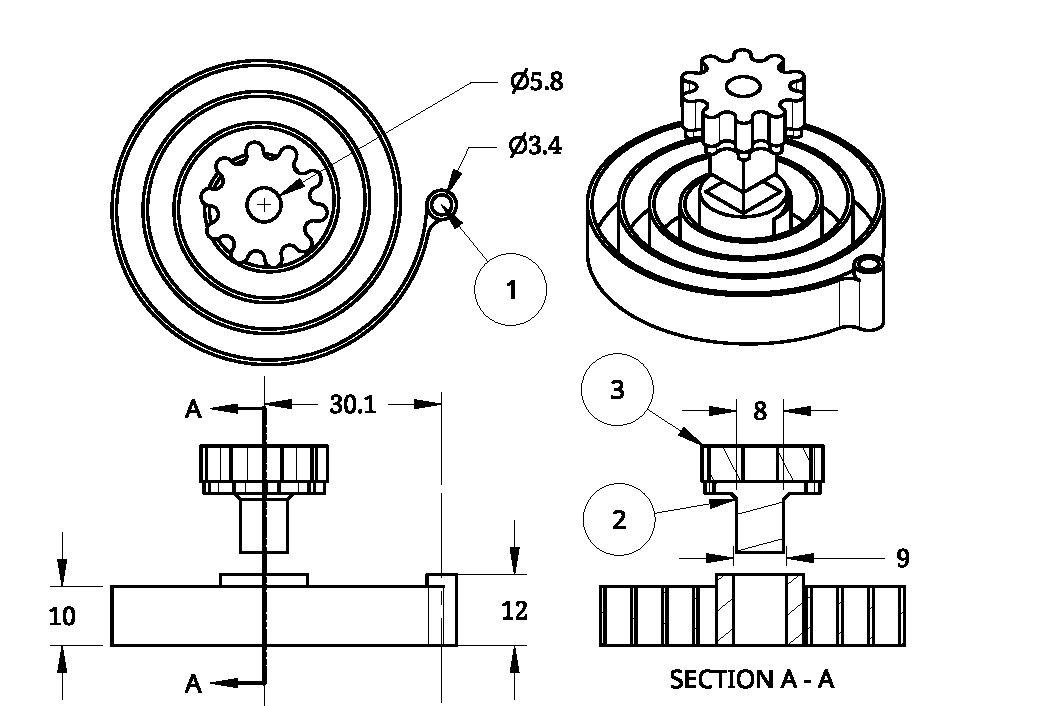
\includegraphics[scale = 1]{pics/DrawingSpring.pdf}
\caption{torsional spring design.}
\end{figure}

\secun{Acceptance test procedure}
Although there is a large software component to the project, the output is purely mechanical. All of the results are therefore pass/fail based on the specification.

\secun{Pictures of final product}
\begin{figure}[H]
\centering
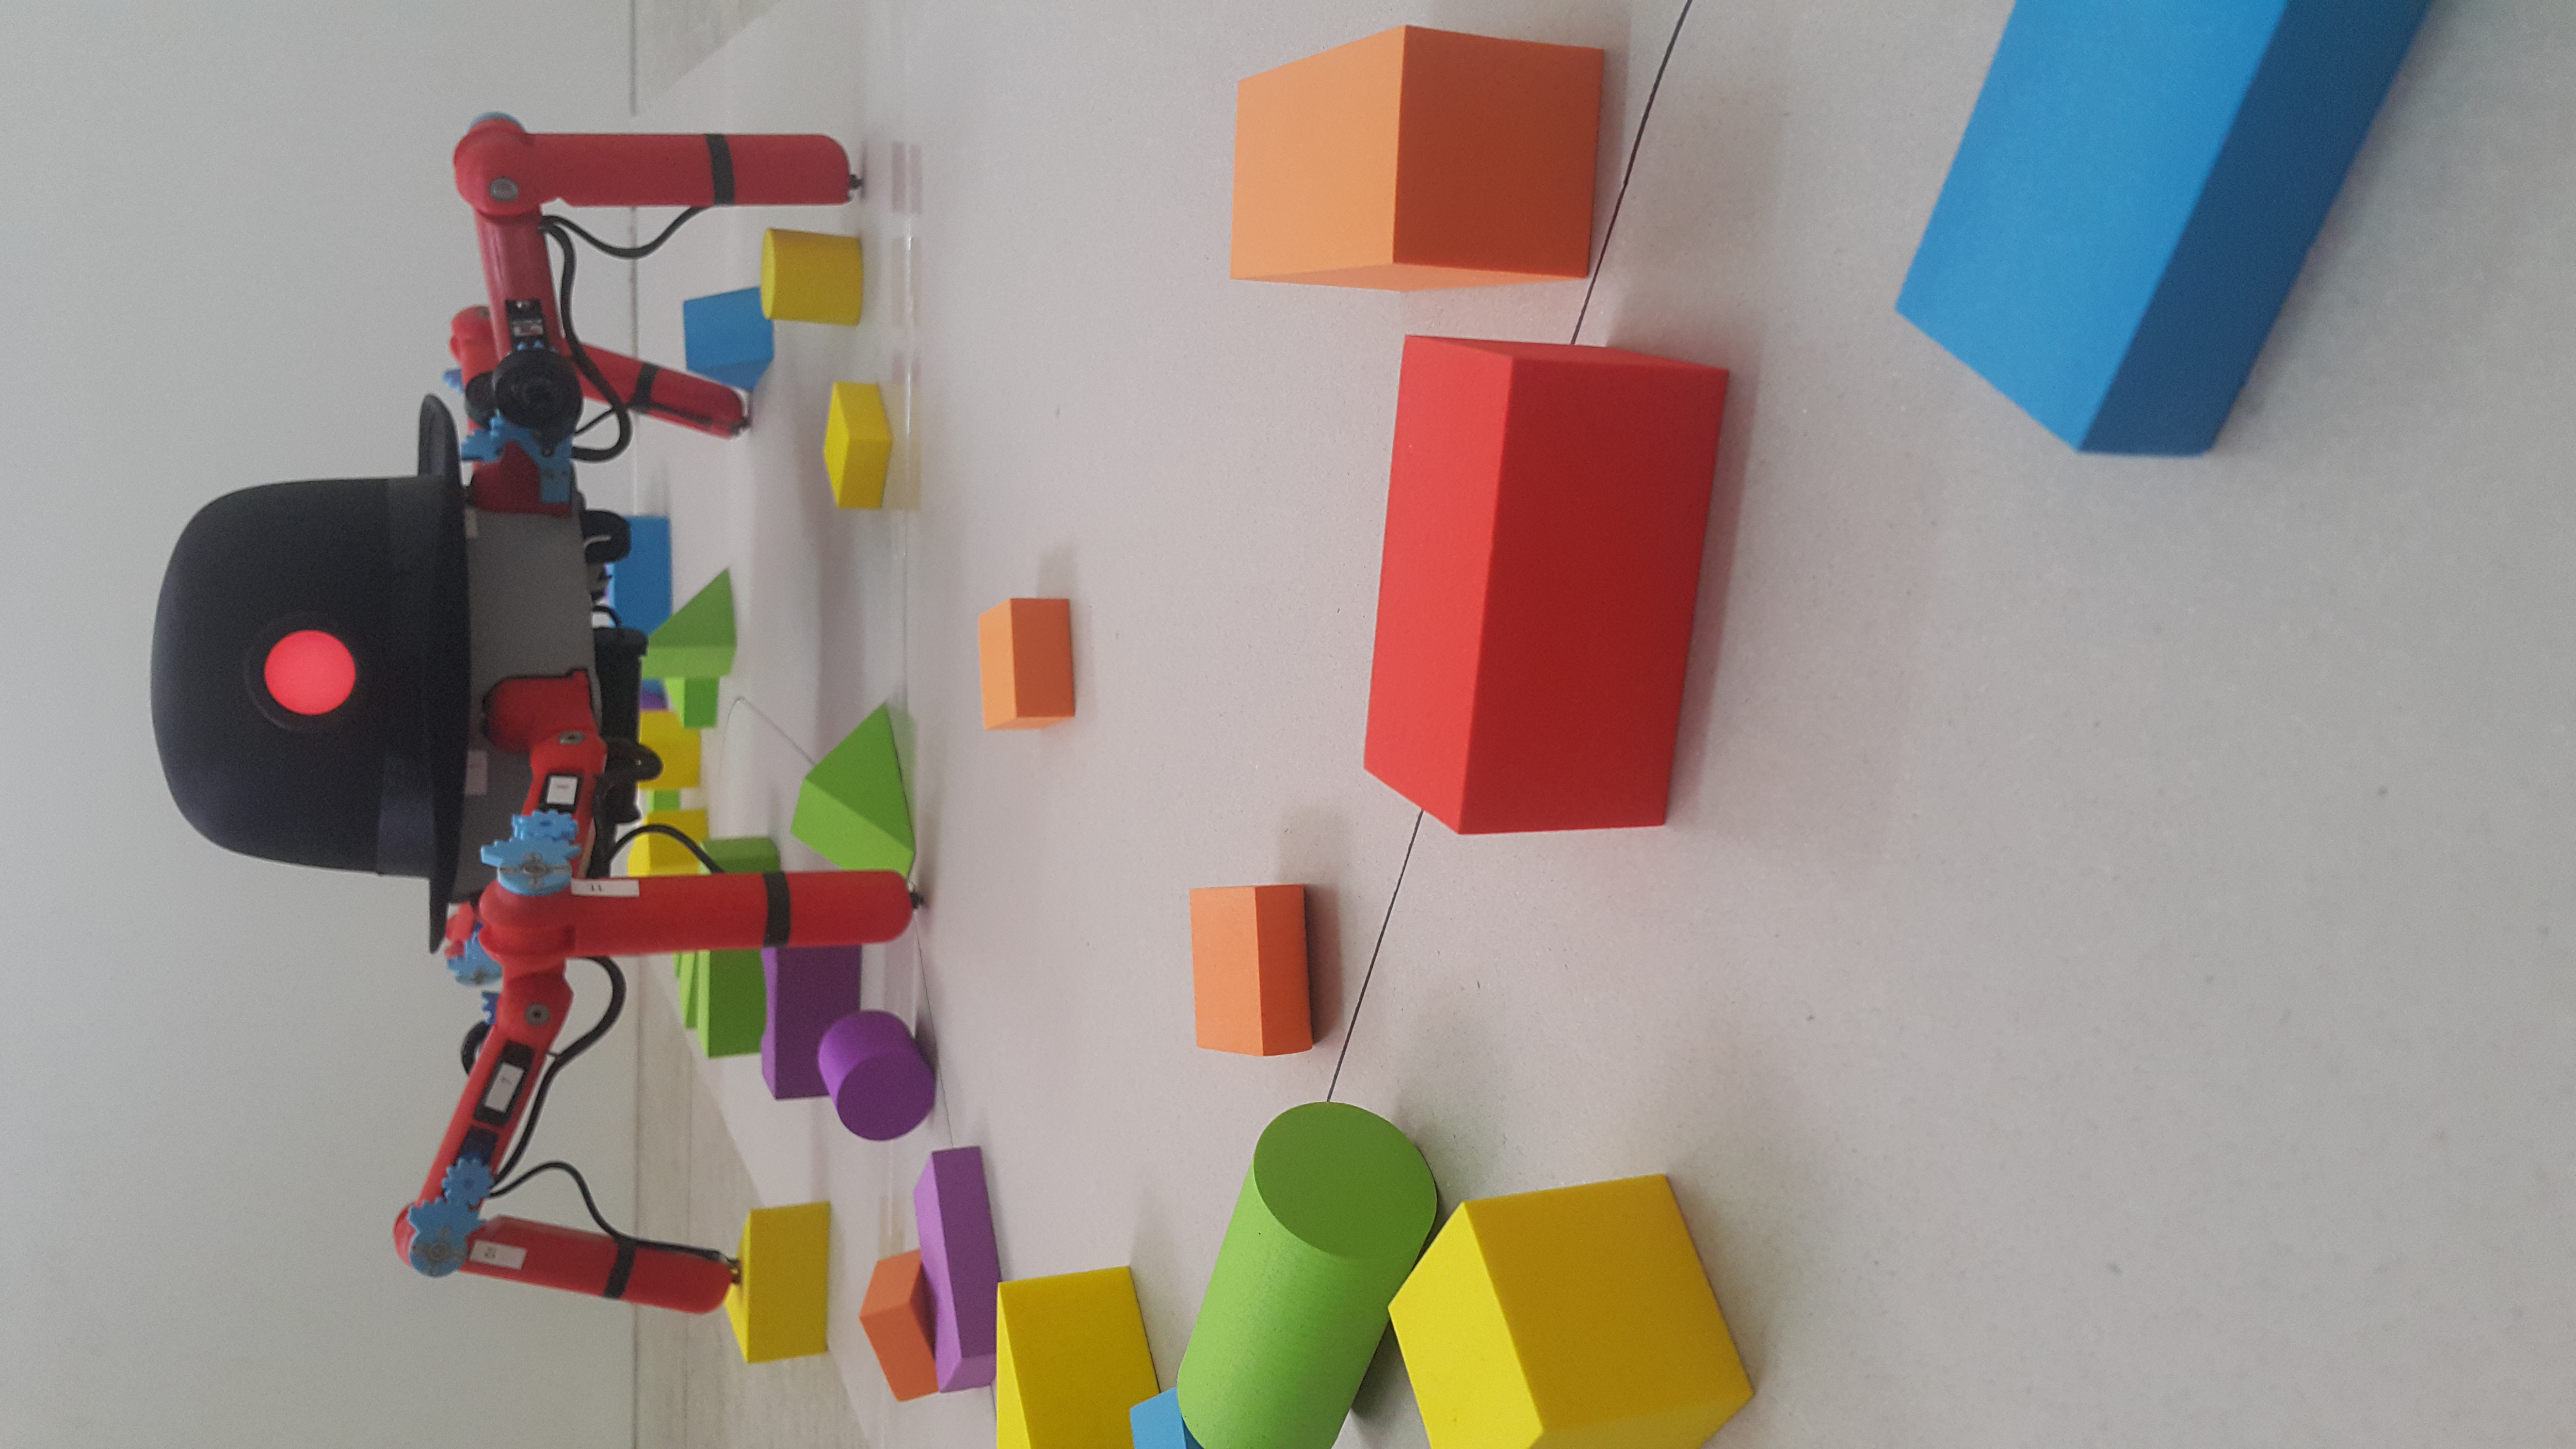
\includegraphics[angle = 270,scale = 0.1]{pics/KRL2.jpg}
\caption{Picture of final product.}
\end{figure}

\secun{User guide}
The robot is simple to operate. Once the batteries are plugged in, it is ready for Bluetooth connection.\\
\secun{List of components cost and suppliers}
This was not collected during the course of the project.\\

\secun{Description of interfacing with other entities}
There are no other entities to be interfaced with.\\

\secun{Flow diagram of software}
\begin{figure}[H]
\centering
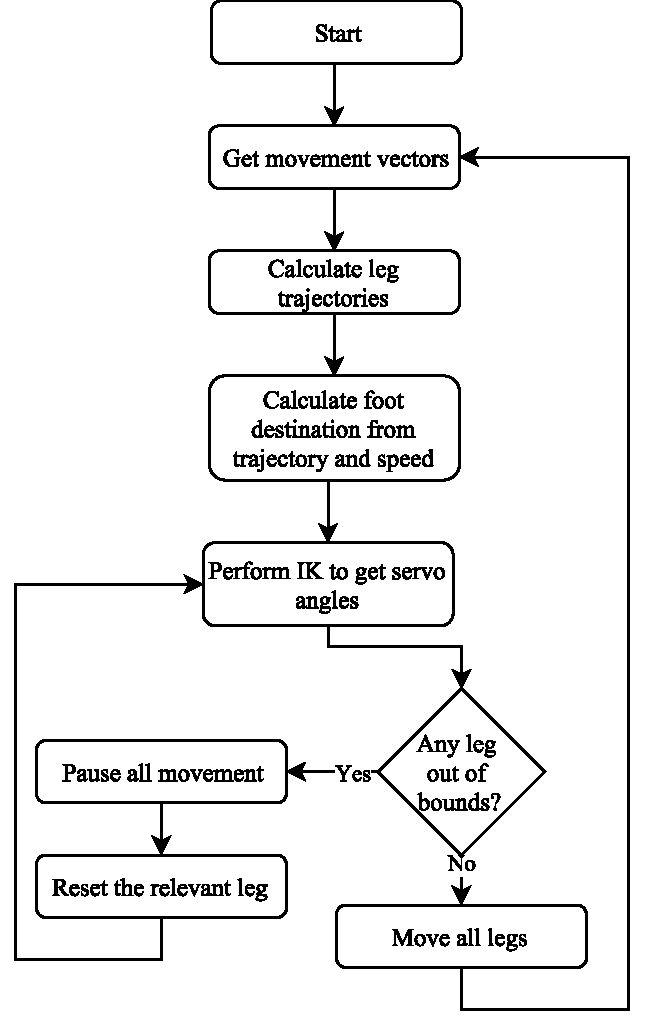
\includegraphics[scale =1]{pics/Soft1.pdf}
\caption{Flow diagram of software.}
\end{figure}

\secun{UML diagrams}
This is not applicable to this project.\\

\secun{Complete source code}
\begin{lstlisting}[language = c]
/**
  ******************************************************************************
  * File Name          : main.c
  * Description        : Main program body
  ******************************************************************************
  ** This notice applies to any and all portions of this file
  * that are not between comment pairs USER CODE BEGIN and
  * USER CODE END. Other portions of this file, whether 
  * inserted by the user or by software development tools
  * are owned by their respective copyright owners.
  *
  * COPYRIGHT(c) 2017 STMicroelectronics
  *
  * Redistribution and use in source and binary forms, with or without modification,
  * are permitted provided that the following conditions are met:
  *   1. Redistributions of source code must retain the above copyright notice,
  *      this list of conditions and the following disclaimer.
  *   2. Redistributions in binary form must reproduce the above copyright notice,
  *      this list of conditions and the following disclaimer in the documentation
  *      and/or other materials provided with the distribution.
  *   3. Neither the name of STMicroelectronics nor the names of its contributors
  *      may be used to endorse or promote products derived from this software
  *      without specific prior written permission.
  *
  * THIS SOFTWARE IS PROVIDED BY THE COPYRIGHT HOLDERS AND CONTRIBUTORS "AS IS"
  * AND ANY EXPRESS OR IMPLIED WARRANTIES, INCLUDING, BUT NOT LIMITED TO, THE
  * IMPLIED WARRANTIES OF MERCHANTABILITY AND FITNESS FOR A PARTICULAR PURPOSE ARE
  * DISCLAIMED. IN NO EVENT SHALL THE COPYRIGHT HOLDER OR CONTRIBUTORS BE LIABLE
  * FOR ANY DIRECT, INDIRECT, INCIDENTAL, SPECIAL, EXEMPLARY, OR CONSEQUENTIAL
  * DAMAGES (INCLUDING, BUT NOT LIMITED TO, PROCUREMENT OF SUBSTITUTE GOODS OR
  * SERVICES; LOSS OF USE, DATA, OR PROFITS; OR BUSINESS INTERRUPTION) HOWEVER
  * CAUSED AND ON ANY THEORY OF LIABILITY, WHETHER IN CONTRACT, STRICT LIABILITY,
  * OR TORT (INCLUDING NEGLIGENCE OR OTHERWISE) ARISING IN ANY WAY OUT OF THE USE
  * OF THIS SOFTWARE, EVEN IF ADVISED OF THE POSSIBILITY OF SUCH DAMAGE.
  *
  ******************************************************************************
  */
/* Includes ------------------------------------------------------------------*/
#include "main.h"
#include "stm32f7xx_hal.h"

/* USER CODE BEGIN Includes */
#include <math.h>
#include <stdbool.h>

/* USER CODE END Includes */

/* Private variables ---------------------------------------------------------*/

I2C_HandleTypeDef hi2c1;

TIM_HandleTypeDef htim6;
TIM_HandleTypeDef htim7;

UART_HandleTypeDef huart1;
UART_HandleTypeDef huart3;

/* USER CODE BEGIN PV */
/* Private variables ---------------------------------------------------------*/
unsigned char RXData[15];																//Array for Bluetooth reception
unsigned char RXDataBuffer[15];													//Temp buffer for above
unsigned char X_Char;																		//Stores received X as Char
unsigned char Y_Char;																		//Stores received Y as Char
unsigned char R_Char;																		//Stores received R as Char
int X_Vect =0;																					//Stores received X as Int
int Y_Vect =0;																					//Stores received Y as Int
int R_Vect =0;																					//Stores received R as Int
int legAngles[3][15];																		//Stores the desired angle for each limb
int legAngles_id[3][15] = {{1, 2, 3, 4, 5,							//Stores the ID of each limb for sorting
											6, 7, 8, 9, 10,
											11, 12, 13, 14, 15},
											{1, 2, 3, 4, 5,										
											6, 7, 8, 9, 10,
											11, 12, 13, 14, 15},
											{1, 2, 3, 4, 5,										
											6, 7, 8, 9, 10,
											11, 12, 13, 14, 15}};

int servoOffset[] = {300,315,300,305,295,								//Array for storing the offset of each servo
											430,460,450,440,442,
											-110,-112,-105,-78,-98};		
int servoMultiplier[] = {	-360,-380,-363,-365,-370,			//Array for storing the multiplier of each servo
													-400,-400,-400,-400,-400,
													480,545,490,460,500};		
int servoCount = 0;																			//Counter used for keeping track of servo interrupts
char servoCountChar[2];
int BTCount = 0;																				//Counter for BlueTooth LED
int newPeriod = 0;

static TIM_HandleTypeDef ServoTimer;
static TIM_HandleTypeDef ServoTimer2;

unsigned char BTRewrite[] = {'X','Y','R','\r'};					//String used for debugging

struct servos {
	int theta;
	int phi;
	int alpha;
};

struct coordinates{
	double x;
	double y;
	double z;
};

struct vectors{
	int X;
	int Y;
	int R;
	bool valid;
};

double rad2deg = 57.29577951308232;
double A_length = 50;
double B_length = 106;
double C_length = 130;
double z_body = 70;
double robotRadius = 90;   

bool resetStatus[5];																		//Array used to store reset status of each leg

double X_Vector = 0;																		//Global movement vectors
double Y_Vector = 0;
double R_Vector = 0;	

double destination[2][5];																//2D array that stores X([0]) and Y([1]) values 
																												//for the destination of each foot
double currentPosition[2][5];														//2D array that stores X and Y values for the 
																												//current position of each foot
double translateLeg[2][5];															//Stores coordinates of joint 1 for each leg.
																												//Replaces TranslateLeg()
bool legAngleFlag = false;															//True when busy writing to legAngles
int bufferLevel;																				//Used to select between levels in buffer
int time = 0;																						//Keeps timing of robot movement for speed calculations
bool BTon = false;																			//Used in program to determine if Bluetooth is connected or not.
//Peripheral pin & port difinitions
#define BTPort 					GPIOE
#define BTLEDPin 				GPIO_PIN_0
#define redLEDPort 			GPIOB
#define redLEDPin 			GPIO_PIN_9
#define greenLEDPort 		GPIOB
#define greenLEDPin 		GPIO_PIN_8
#define servoPowerPort	GPIOC
#define servoPowerPin		GPIO_PIN_9

//Servo pin & port definitions
#define servo1Pin 		GPIO_PIN_12
#define servo1Port 		GPIOB
#define servo2Pin 		GPIO_PIN_13
#define servo2Port 		GPIOB
#define servo3Pin 		GPIO_PIN_14
#define servo3Port 		GPIOB
#define servo4Pin 		GPIO_PIN_15
#define servo4Port 		GPIOB
#define servo5Pin 		GPIO_PIN_8
#define servo5Port 		GPIOD
#define servo6Pin 		GPIO_PIN_9
#define servo6Port 		GPIOD
#define servo7Pin 		GPIO_PIN_10
#define servo7Port 		GPIOD
#define servo8Pin 		GPIO_PIN_11
#define servo8Port 		GPIOD
#define servo9Pin 		GPIO_PIN_12
#define servo9Port 		GPIOD
#define servo10Pin 		GPIO_PIN_13
#define servo10Port 	GPIOD
#define servo11Pin 		GPIO_PIN_14
#define servo11Port 	GPIOD
#define servo12Pin 		GPIO_PIN_15
#define servo12Port 	GPIOD
#define servo13Pin 		GPIO_PIN_6
#define servo13Port 	GPIOC
#define servo14Pin 		GPIO_PIN_7
#define servo14Port 	GPIOC
#define servo15Pin 		GPIO_PIN_8
#define servo15Port 	GPIOC

uint16_t servoPinArray[] ={	servo1Pin, servo2Pin, servo3Pin,
														servo4Pin, servo5Pin, servo6Pin,
														servo7Pin, servo8Pin, servo9Pin,
														servo10Pin, servo11Pin, servo12Pin,
														servo13Pin, servo14Pin, servo15Pin};

GPIO_TypeDef * servoPortArray[] = {	servo1Port, servo2Port, servo3Port,
																		servo4Port, servo5Port, servo6Port,
																		servo7Port, servo8Port, servo9Port,
																		servo10Port, servo11Port, servo12Port,
																		servo13Port, servo14Port, servo15Port};
/* USER CODE END PV */

/* Private function prototypes -----------------------------------------------*/
void SystemClock_Config(void);
static void MX_GPIO_Init(void);
static void MX_USART3_UART_Init(void);
static void MX_USART1_UART_Init(void);
static void MX_TIM6_Init(void);
static void MX_TIM7_Init(void);
static void MX_I2C1_Init(void);

/* USER CODE BEGIN PFP */
/* Private function prototypes -----------------------------------------------*/
void Debug(char *Array, int count);														//Sends something to UART1 for debugging
void HAL_UART_ErrorCallback(UART_HandleTypeDef *huart);				//Sends error message with Debug()
void SetupTimers(void);																				//Configure timers 6 and 7 for use in servo control
void Sort(void);																							//Sorts timer values into ascending order
void SetServo(int servo, int degrees);												//Sets the timer value for a servo from a degree value
struct servos IK( struct coordinates input);									//Inverse Kinematics function
bool CheckBounds(struct servos leg);													//Check if legs need to be reset
struct coordinates Rotate(double x, double y, double angle);	//Rotate coordinates about an angle
void TranslateLeg(void);																			//Generates constants at beginning of program
struct coordinates Vector(double x, double y, int leg, bool offset, double r);
void StartPosition(void);																			//Resets robot to default position
void HAL_UART_RxCpltCallback(UART_HandleTypeDef *huart);			//ISR for when bluetooth communication is received.
void BTDecrypt(void);																//Resturns vectors sent from android
void ServoUpdate(void);																				//Moves entire buffer over at once to servos
void Delay(int a);																						//Delays program for a cycles of 20ms
void ResetLeg(int leg);																				//Moves the specified leg back to its origin
void DestinationUpdate(int leg);															//Calculates the new destination from the input vectors and the current values

/* USER CODE END PFP */

/* USER CODE BEGIN 0 */

/* USER CODE END 0 */

int main(void)
{

  /* USER CODE BEGIN 1 */

  /* USER CODE END 1 */

  /* MCU Configuration----------------------------------------------------------*/

  /* Reset of all peripherals, Initializes the Flash interface and the Systick. */
  HAL_Init();

  /* USER CODE BEGIN Init */

  /* USER CODE END Init */

  /* Configure the system clock */
  SystemClock_Config();

  /* USER CODE BEGIN SysInit */

  /* USER CODE END SysInit */

  /* Initialize all configured peripherals */
  MX_GPIO_Init();
  MX_USART3_UART_Init();
  MX_USART1_UART_Init();
  MX_TIM6_Init();
  MX_TIM7_Init();
  MX_I2C1_Init();

  /* USER CODE BEGIN 2 */
	SetupTimers();
	StartPosition();

	TranslateLeg();

	Debug("Init done",9);

  /* USER CODE END 2 */

  /* Infinite loop */
  /* USER CODE BEGIN WHILE */
	Debug("Entering main loop",18);
	HAL_UART_Receive_IT(&huart3,RXDataBuffer,15);											//Receive commands via bluetooth in interrupt mode
  while (1)
  {
  /* USER CODE END WHILE */

  /* USER CODE BEGIN 3 */
		//Turn off all LEDs except red
		HAL_GPIO_WritePin(BTPort,BTLEDPin,GPIO_PIN_SET);
		HAL_GPIO_WritePin(greenLEDPort,greenLEDPin,GPIO_PIN_SET);
		HAL_GPIO_WritePin(redLEDPort,redLEDPin,GPIO_PIN_RESET);
		
		Debug("Waiting for Bluetooth...",24);
		
		while (BTon == false)
		{
			//Wait here for connection
		}
		//Turn off all LEDs except blue
		HAL_GPIO_WritePin(BTPort,BTLEDPin,GPIO_PIN_RESET);
		HAL_GPIO_WritePin(greenLEDPort,greenLEDPin,GPIO_PIN_SET);
		HAL_GPIO_WritePin(redLEDPort,redLEDPin,GPIO_PIN_SET);
		Debug("Turning on servos...",20);
		//Move servos to home position
		StartPosition();
		//Turn on power to servos
		HAL_GPIO_WritePin(servoPowerPort,servoPowerPin,GPIO_PIN_SET);
		//Delay for 1 second to get things started
		Delay(10);
		//Put legs in the 0,0,50 position one at a time
		for (int leg = 1; leg <6; leg++)
		{
			struct coordinates leg_Vector = Vector(0,0,leg,true,0);
			leg_Vector.z = 50;			//Lift legs above ground
			struct servos leg_servo = IK(leg_Vector);
			
			SetServo(leg,leg_servo.theta);
			SetServo(leg+5,leg_servo.phi);
			SetServo(leg+10,leg_servo.alpha);
			ServoUpdate();
			Delay(10);
		}
		//Slowly raise the body
		for (int height = 50 ; height >0 ; --height)
		{
			for (int leg = 1; leg <6; leg++)
			{
				struct coordinates leg_Vector = Vector(0,0,leg,true,0);
				leg_Vector.z = height;			//Lift legs above ground
				struct servos leg_servo = IK(leg_Vector);
				
				SetServo(leg,leg_servo.theta);
				SetServo(leg+5,leg_servo.phi);
				SetServo(leg+10,leg_servo.alpha);
				ServoUpdate();
			}
			Delay(2);
		}
		//Turn off all LEDs except green
		HAL_GPIO_WritePin(BTPort,BTLEDPin,GPIO_PIN_SET);
		HAL_GPIO_WritePin(greenLEDPort,greenLEDPin,GPIO_PIN_RESET);
		HAL_GPIO_WritePin(redLEDPort,redLEDPin,GPIO_PIN_SET);
		Debug("Ready...",8);
		
		//This is the main part that executes while the bluetooth is connected
		while(BTon)
		{
			//Get the vectors from the last transmitted message
			BTDecrypt();
			//Perform inverse kinematics
			for (int leg = 1; leg <6; leg++)
			{
//				struct coordinates leg_Vector = Vector(-X_Vect,-Y_Vect,leg,true);  //!!!!!!!!!This does not accumulate!!!!!!!!!!!!!!!!!!!!!!			
				DestinationUpdate(leg);
				struct coordinates leg_Vector;
				leg_Vector.x = currentPosition[0][leg-1];
				leg_Vector.y = currentPosition[1][leg-1];
				leg_Vector.z = 0;
				struct servos leg_servo = IK(leg_Vector);
				//Check if this is out ouf bounds
				if (CheckBounds(leg_servo))
				{
					resetStatus[leg-1] = true;
				}else{
					resetStatus[leg-1] = false;
				}
				SetServo(leg,leg_servo.theta);
				SetServo(leg+5,leg_servo.phi);
				SetServo(leg+10,leg_servo.alpha);
			}
			//Reset legs if necessary
			for (int leg = 1; leg < 6; leg++)
			{
				if (resetStatus[leg-1] == true)
				{
					//Turn on all LEDs (white)
					HAL_GPIO_WritePin(BTPort,BTLEDPin,GPIO_PIN_RESET);
					HAL_GPIO_WritePin(greenLEDPort,greenLEDPin,GPIO_PIN_RESET);
					HAL_GPIO_WritePin(redLEDPort,redLEDPin,GPIO_PIN_RESET);
					//Reset leg
					ResetLeg(leg);
				}
			}
			//Move the legs to where we want them
			ServoUpdate();
			//Turn off all LEDs except green
			HAL_GPIO_WritePin(BTPort,BTLEDPin,GPIO_PIN_SET);
			HAL_GPIO_WritePin(greenLEDPort,greenLEDPin,GPIO_PIN_RESET);
			HAL_GPIO_WritePin(redLEDPort,redLEDPin,GPIO_PIN_SET);
		}
		
		

  }
  /* USER CODE END 3 */

}

/** System Clock Configuration
*/
void SystemClock_Config(void)
{

  RCC_OscInitTypeDef RCC_OscInitStruct;
  RCC_ClkInitTypeDef RCC_ClkInitStruct;
  RCC_PeriphCLKInitTypeDef PeriphClkInitStruct;

    /**Configure the main internal regulator output voltage 
    */
  __HAL_RCC_PWR_CLK_ENABLE();

  __HAL_PWR_VOLTAGESCALING_CONFIG(PWR_REGULATOR_VOLTAGE_SCALE1);

    /**Initializes the CPU, AHB and APB busses clocks 
    */
  RCC_OscInitStruct.OscillatorType = RCC_OSCILLATORTYPE_HSE;
  RCC_OscInitStruct.HSEState = RCC_HSE_ON;
  RCC_OscInitStruct.PLL.PLLState = RCC_PLL_ON;
  RCC_OscInitStruct.PLL.PLLSource = RCC_PLLSOURCE_HSE;
  RCC_OscInitStruct.PLL.PLLM = 10;
  RCC_OscInitStruct.PLL.PLLN = 216;
  RCC_OscInitStruct.PLL.PLLP = RCC_PLLP_DIV2;
  RCC_OscInitStruct.PLL.PLLQ = 2;
  if (HAL_RCC_OscConfig(&RCC_OscInitStruct) != HAL_OK)
  {
    _Error_Handler(__FILE__, __LINE__);
  }

    /**Activate the Over-Drive mode 
    */
  if (HAL_PWREx_EnableOverDrive() != HAL_OK)
  {
    _Error_Handler(__FILE__, __LINE__);
  }

    /**Initializes the CPU, AHB and APB busses clocks 
    */
  RCC_ClkInitStruct.ClockType = RCC_CLOCKTYPE_HCLK|RCC_CLOCKTYPE_SYSCLK
                              |RCC_CLOCKTYPE_PCLK1|RCC_CLOCKTYPE_PCLK2;
  RCC_ClkInitStruct.SYSCLKSource = RCC_SYSCLKSOURCE_PLLCLK;
  RCC_ClkInitStruct.AHBCLKDivider = RCC_SYSCLK_DIV1;
  RCC_ClkInitStruct.APB1CLKDivider = RCC_HCLK_DIV4;
  RCC_ClkInitStruct.APB2CLKDivider = RCC_HCLK_DIV2;

  if (HAL_RCC_ClockConfig(&RCC_ClkInitStruct, FLASH_LATENCY_7) != HAL_OK)
  {
    _Error_Handler(__FILE__, __LINE__);
  }

  PeriphClkInitStruct.PeriphClockSelection = RCC_PERIPHCLK_USART1|RCC_PERIPHCLK_USART3
                              |RCC_PERIPHCLK_I2C1;
  PeriphClkInitStruct.Usart1ClockSelection = RCC_USART1CLKSOURCE_PCLK2;
  PeriphClkInitStruct.Usart3ClockSelection = RCC_USART3CLKSOURCE_PCLK1;
  PeriphClkInitStruct.I2c1ClockSelection = RCC_I2C1CLKSOURCE_PCLK1;
  if (HAL_RCCEx_PeriphCLKConfig(&PeriphClkInitStruct) != HAL_OK)
  {
    _Error_Handler(__FILE__, __LINE__);
  }

    /**Configure the Systick interrupt time 
    */
  HAL_SYSTICK_Config(HAL_RCC_GetHCLKFreq()/1000);

    /**Configure the Systick 
    */
  HAL_SYSTICK_CLKSourceConfig(SYSTICK_CLKSOURCE_HCLK);

  /* SysTick_IRQn interrupt configuration */
  HAL_NVIC_SetPriority(SysTick_IRQn, 0, 0);
}

/* I2C1 init function */
static void MX_I2C1_Init(void)
{

  hi2c1.Instance = I2C1;
  hi2c1.Init.Timing = 0x20404768;
  hi2c1.Init.OwnAddress1 = 0;
  hi2c1.Init.AddressingMode = I2C_ADDRESSINGMODE_7BIT;
  hi2c1.Init.DualAddressMode = I2C_DUALADDRESS_DISABLE;
  hi2c1.Init.OwnAddress2 = 0;
  hi2c1.Init.OwnAddress2Masks = I2C_OA2_NOMASK;
  hi2c1.Init.GeneralCallMode = I2C_GENERALCALL_DISABLE;
  hi2c1.Init.NoStretchMode = I2C_NOSTRETCH_DISABLE;
  if (HAL_I2C_Init(&hi2c1) != HAL_OK)
  {
    _Error_Handler(__FILE__, __LINE__);
  }

    /**Configure Analogue filter 
    */
  if (HAL_I2CEx_ConfigAnalogFilter(&hi2c1, I2C_ANALOGFILTER_ENABLE) != HAL_OK)
  {
    _Error_Handler(__FILE__, __LINE__);
  }

    /**Configure Digital filter 
    */
  if (HAL_I2CEx_ConfigDigitalFilter(&hi2c1, 0) != HAL_OK)
  {
    _Error_Handler(__FILE__, __LINE__);
  }

}

/* TIM6 init function */
static void MX_TIM6_Init(void)
{

  TIM_MasterConfigTypeDef sMasterConfig;

  htim6.Instance = TIM6;
  htim6.Init.Prescaler = 0;
  htim6.Init.CounterMode = TIM_COUNTERMODE_UP;
  htim6.Init.Period = 0;
  htim6.Init.AutoReloadPreload = TIM_AUTORELOAD_PRELOAD_DISABLE;
  if (HAL_TIM_Base_Init(&htim6) != HAL_OK)
  {
    _Error_Handler(__FILE__, __LINE__);
  }

  sMasterConfig.MasterOutputTrigger = TIM_TRGO_RESET;
  sMasterConfig.MasterSlaveMode = TIM_MASTERSLAVEMODE_DISABLE;
  if (HAL_TIMEx_MasterConfigSynchronization(&htim6, &sMasterConfig) != HAL_OK)
  {
    _Error_Handler(__FILE__, __LINE__);
  }

}

/* TIM7 init function */
static void MX_TIM7_Init(void)
{

  TIM_MasterConfigTypeDef sMasterConfig;

  htim7.Instance = TIM7;
  htim7.Init.Prescaler = 0;
  htim7.Init.CounterMode = TIM_COUNTERMODE_UP;
  htim7.Init.Period = 0;
  htim7.Init.AutoReloadPreload = TIM_AUTORELOAD_PRELOAD_DISABLE;
  if (HAL_TIM_Base_Init(&htim7) != HAL_OK)
  {
    _Error_Handler(__FILE__, __LINE__);
  }

  sMasterConfig.MasterOutputTrigger = TIM_TRGO_RESET;
  sMasterConfig.MasterSlaveMode = TIM_MASTERSLAVEMODE_DISABLE;
  if (HAL_TIMEx_MasterConfigSynchronization(&htim7, &sMasterConfig) != HAL_OK)
  {
    _Error_Handler(__FILE__, __LINE__);
  }

}

/* USART1 init function */
static void MX_USART1_UART_Init(void)
{

  huart1.Instance = USART1;
  huart1.Init.BaudRate = 115200;
  huart1.Init.WordLength = UART_WORDLENGTH_8B;
  huart1.Init.StopBits = UART_STOPBITS_1;
  huart1.Init.Parity = UART_PARITY_NONE;
  huart1.Init.Mode = UART_MODE_TX_RX;
  huart1.Init.HwFlowCtl = UART_HWCONTROL_NONE;
  huart1.Init.OverSampling = UART_OVERSAMPLING_16;
  huart1.Init.OneBitSampling = UART_ONE_BIT_SAMPLE_DISABLE;
  huart1.AdvancedInit.AdvFeatureInit = UART_ADVFEATURE_NO_INIT;
  if (HAL_UART_Init(&huart1) != HAL_OK)
  {
    _Error_Handler(__FILE__, __LINE__);
  }

}

/* USART3 init function */
static void MX_USART3_UART_Init(void)
{

  huart3.Instance = USART3;
  huart3.Init.BaudRate = 9600;
  huart3.Init.WordLength = UART_WORDLENGTH_8B;
  huart3.Init.StopBits = UART_STOPBITS_1;
  huart3.Init.Parity = UART_PARITY_NONE;
  huart3.Init.Mode = UART_MODE_TX_RX;
  huart3.Init.HwFlowCtl = UART_HWCONTROL_NONE;
  huart3.Init.OverSampling = UART_OVERSAMPLING_16;
  huart3.Init.OneBitSampling = UART_ONE_BIT_SAMPLE_DISABLE;
  huart3.AdvancedInit.AdvFeatureInit = UART_ADVFEATURE_NO_INIT;
  if (HAL_UART_Init(&huart3) != HAL_OK)
  {
    _Error_Handler(__FILE__, __LINE__);
  }

}

/** Configure pins as 
        * Analog 
        * Input 
        * Output
        * EVENT_OUT
        * EXTI
*/
static void MX_GPIO_Init(void)
{

  GPIO_InitTypeDef GPIO_InitStruct;

  /* GPIO Ports Clock Enable */
  __HAL_RCC_GPIOH_CLK_ENABLE();
  __HAL_RCC_GPIOC_CLK_ENABLE();
  __HAL_RCC_GPIOA_CLK_ENABLE();
  __HAL_RCC_GPIOB_CLK_ENABLE();
  __HAL_RCC_GPIOD_CLK_ENABLE();
  __HAL_RCC_GPIOE_CLK_ENABLE();

  /*Configure GPIO pin Output Level */
  HAL_GPIO_WritePin(GPIOC, GPIO_PIN_1|GPIO_PIN_6|GPIO_PIN_7|GPIO_PIN_8 
                          |GPIO_PIN_9, GPIO_PIN_RESET);

  /*Configure GPIO pin Output Level */
  HAL_GPIO_WritePin(GPIOA, GPIO_PIN_1, GPIO_PIN_RESET);

  /*Configure GPIO pin Output Level */
  HAL_GPIO_WritePin(GPIOB, GPIO_PIN_1|GPIO_PIN_12|GPIO_PIN_13|GPIO_PIN_14 
                          |GPIO_PIN_15|GPIO_PIN_8|GPIO_PIN_9, GPIO_PIN_RESET);

  /*Configure GPIO pin Output Level */
  HAL_GPIO_WritePin(GPIOD, GPIO_PIN_8|GPIO_PIN_9|GPIO_PIN_10|GPIO_PIN_11 
                          |GPIO_PIN_12|GPIO_PIN_13|GPIO_PIN_14|GPIO_PIN_15 
                          |GPIO_PIN_1, GPIO_PIN_RESET);

  /*Configure GPIO pin Output Level */
  HAL_GPIO_WritePin(GPIOE, GPIO_PIN_0|GPIO_PIN_1, GPIO_PIN_RESET);

  /*Configure GPIO pins : PC1 PC6 PC7 PC8 
                           PC9 */
  GPIO_InitStruct.Pin = GPIO_PIN_1|GPIO_PIN_6|GPIO_PIN_7|GPIO_PIN_8 
                          |GPIO_PIN_9;
  GPIO_InitStruct.Mode = GPIO_MODE_OUTPUT_PP;
  GPIO_InitStruct.Pull = GPIO_NOPULL;
  GPIO_InitStruct.Speed = GPIO_SPEED_FREQ_LOW;
  HAL_GPIO_Init(GPIOC, &GPIO_InitStruct);

  /*Configure GPIO pin : PA1 */
  GPIO_InitStruct.Pin = GPIO_PIN_1;
  GPIO_InitStruct.Mode = GPIO_MODE_OUTPUT_PP;
  GPIO_InitStruct.Pull = GPIO_NOPULL;
  GPIO_InitStruct.Speed = GPIO_SPEED_FREQ_LOW;
  HAL_GPIO_Init(GPIOA, &GPIO_InitStruct);

  /*Configure GPIO pins : PA4 PA5 PA6 PA7 */
  GPIO_InitStruct.Pin = GPIO_PIN_4|GPIO_PIN_5|GPIO_PIN_6|GPIO_PIN_7;
  GPIO_InitStruct.Mode = GPIO_MODE_INPUT;
  GPIO_InitStruct.Pull = GPIO_NOPULL;
  HAL_GPIO_Init(GPIOA, &GPIO_InitStruct);

  /*Configure GPIO pin : PC4 */
  GPIO_InitStruct.Pin = GPIO_PIN_4;
  GPIO_InitStruct.Mode = GPIO_MODE_INPUT;
  GPIO_InitStruct.Pull = GPIO_NOPULL;
  HAL_GPIO_Init(GPIOC, &GPIO_InitStruct);

  /*Configure GPIO pins : PB1 PB12 PB13 PB14 
                           PB15 PB8 PB9 */
  GPIO_InitStruct.Pin = GPIO_PIN_1|GPIO_PIN_12|GPIO_PIN_13|GPIO_PIN_14 
                          |GPIO_PIN_15|GPIO_PIN_8|GPIO_PIN_9;
  GPIO_InitStruct.Mode = GPIO_MODE_OUTPUT_PP;
  GPIO_InitStruct.Pull = GPIO_NOPULL;
  GPIO_InitStruct.Speed = GPIO_SPEED_FREQ_LOW;
  HAL_GPIO_Init(GPIOB, &GPIO_InitStruct);

  /*Configure GPIO pins : PD8 PD9 PD10 PD11 
                           PD12 PD13 PD14 PD15 
                           PD1 */
  GPIO_InitStruct.Pin = GPIO_PIN_8|GPIO_PIN_9|GPIO_PIN_10|GPIO_PIN_11 
                          |GPIO_PIN_12|GPIO_PIN_13|GPIO_PIN_14|GPIO_PIN_15 
                          |GPIO_PIN_1;
  GPIO_InitStruct.Mode = GPIO_MODE_OUTPUT_PP;
  GPIO_InitStruct.Pull = GPIO_NOPULL;
  GPIO_InitStruct.Speed = GPIO_SPEED_FREQ_LOW;
  HAL_GPIO_Init(GPIOD, &GPIO_InitStruct);

  /*Configure GPIO pins : PE0 PE1 */
  GPIO_InitStruct.Pin = GPIO_PIN_0|GPIO_PIN_1;
  GPIO_InitStruct.Mode = GPIO_MODE_OUTPUT_PP;
  GPIO_InitStruct.Pull = GPIO_NOPULL;
  GPIO_InitStruct.Speed = GPIO_SPEED_FREQ_LOW;
  HAL_GPIO_Init(GPIOE, &GPIO_InitStruct);

}

/* USER CODE BEGIN 4 */

/**
  * @brief  This function sends a string to UART1 to be received in a terminal
	* @param  *Array is a pointer to the string
						count is an int equal to the number of characters in the string
  * @retval None
  */
void Debug(char *Array, int count)
{
	uint8_t TXBuffer[count+1];
	for(int i = 0; i!=count;i++)
	{
		TXBuffer[i] = Array[i];
	}		
	
	TXBuffer[count] ='\r';
	TXBuffer[count+1] ='\n';
	HAL_UART_Transmit(&huart1,TXBuffer,count+2,10);
}

/**
  * @brief  This function is executed in the case of an error with the UART modules
	* @param  *huart is a handle of the UART module in question
  * @retval None
  */
void HAL_UART_ErrorCallback(UART_HandleTypeDef *huart)
{
	if (huart == &huart3)
	{
		Debug("Bluetooth Error",15);
	}else if (huart == &huart1)
	{
		Debug("Serial Error",12);
	}else{
		Debug("UART error",10);
	}
	
}

/**
  * @brief  This function configures the timers used in generating the servo signals
	* @param  None
  * @retval None
  */
void SetupTimers(void)
{
	//Timer 6
	//50Hz Interrupt
	ServoTimer.Instance =TIM6;
	ServoTimer.Init.Prescaler =40000;
	ServoTimer.Init.CounterMode = TIM_COUNTERMODE_UP;
	ServoTimer.Init.Period =54;
	ServoTimer.Init.RepetitionCounter = 0;
	HAL_TIM_Base_Init(&ServoTimer);
	HAL_TIM_Base_Start_IT(&ServoTimer);
	
	//Timer 7
	//Variable frequency interrupt
	htim7.Instance =TIM7;
	htim7.Init.Prescaler =1000;
	htim7.Init.CounterMode = TIM_COUNTERMODE_UP;
	htim7.Init.Period =160;
	htim7.Init.RepetitionCounter = 0;
	HAL_TIM_Base_Init(&htim7);
	HAL_TIM_Base_Start_IT(&htim7);
}
	

/** @brief Function for sorting the desired leg angles into ascending order 
						to make timer functions simpler
  * @param None
  * @retval None */
void Sort(void)
{
	for(int i = 0;i<15;i++)
	{
		for(int j = i+1;j<15;j++)
		{
			if(legAngles[0][i] > legAngles[0][j])
			{
				//swop the angles
				int a = legAngles[0][i];
				legAngles[0][i] = legAngles[0][j];
				legAngles[0][j] = a;
				//now swop the index
				a = legAngles_id[0][i];
				legAngles_id[0][i] = legAngles_id[0][j];
				legAngles_id[0][j] = a;
			}
		}
	}
}

/**
  * @brief  This function executes when a timer interrupts. It is used to generate servo signals
	* @param  *htim is a handle of the timer module that triggered the interrupt
  * @retval None
  */
void HAL_TIM_PeriodElapsedCallback(TIM_HandleTypeDef *htim)
	{
		
		if(htim == &htim7){
			if(legAngleFlag == true)
			{
				bufferLevel = 2;
			}else{
				bufferLevel = 1;
			}
			//Turn off
			++servoCount;			
			if (servoCount < 15)
			{
				newPeriod = (legAngles[bufferLevel][servoCount]- legAngles[bufferLevel][servoCount-1]);
				
				while (newPeriod == 0)
				{
					HAL_GPIO_WritePin(servoPortArray[legAngles_id[bufferLevel][servoCount-1]-1] ,servoPinArray[legAngles_id[bufferLevel][servoCount-1]-1],GPIO_PIN_RESET);
					++servoCount;
					newPeriod = (legAngles[bufferLevel][servoCount]- legAngles[bufferLevel][servoCount-1]);
				}
				//Adjust for time lost in this subroutine
				if (newPeriod>1)
				{
					--newPeriod;
				}
				if (newPeriod < 0 || newPeriod > 400)
				{
					newPeriod = 0;
				}
				TIM7->ARR = (newPeriod);
				HAL_GPIO_WritePin(servoPortArray[legAngles_id[bufferLevel][servoCount-1]-1] ,servoPinArray[legAngles_id[bufferLevel][servoCount-1]-1],GPIO_PIN_RESET);
			}else{
				//Turn off servo 15
				HAL_GPIO_WritePin(servoPortArray[legAngles_id[bufferLevel][14]-1] ,servoPinArray[legAngles_id[bufferLevel][14]-1],GPIO_PIN_RESET);
				//Stop the timer for the rest of the cycle
				HAL_TIM_Base_Stop(&htim7);
				if (servoCount != 0xF)
				{
					Debug("servoCount Error",16);
				}
				servoCount = 0;
			}
		}else if (htim == &htim6)
		{
			servoCount = 0;
			++time;
			//50Hz Interrupt
			//Turn all on
			HAL_GPIO_WritePin(servo1Port,servo1Pin,GPIO_PIN_SET);
			HAL_GPIO_WritePin(servo2Port,servo2Pin,GPIO_PIN_SET);
			HAL_GPIO_WritePin(servo3Port,servo3Pin,GPIO_PIN_SET);
			HAL_GPIO_WritePin(servo4Port,servo4Pin,GPIO_PIN_SET);
			HAL_GPIO_WritePin(servo5Port,servo5Pin,GPIO_PIN_SET);
			HAL_GPIO_WritePin(servo6Port,servo6Pin,GPIO_PIN_SET);
			HAL_GPIO_WritePin(servo7Port,servo7Pin,GPIO_PIN_SET);
			HAL_GPIO_WritePin(servo8Port,servo8Pin,GPIO_PIN_SET);
			HAL_GPIO_WritePin(servo9Port,servo9Pin,GPIO_PIN_SET);
			HAL_GPIO_WritePin(servo10Port,servo10Pin,GPIO_PIN_SET);
			HAL_GPIO_WritePin(servo11Port,servo11Pin,GPIO_PIN_SET);
			HAL_GPIO_WritePin(servo12Port,servo12Pin,GPIO_PIN_SET);
			HAL_GPIO_WritePin(servo13Port,servo13Pin,GPIO_PIN_SET);
			HAL_GPIO_WritePin(servo14Port,servo14Pin,GPIO_PIN_SET);
			HAL_GPIO_WritePin(servo15Port,servo15Pin,GPIO_PIN_SET);
			

			if(legAngleFlag == true)
			{
				bufferLevel = 2;
			}else{
				bufferLevel = 1;
			}
			//Set period for 1st servo
			newPeriod = legAngles[bufferLevel][servoCount];
			if (newPeriod < 0 || newPeriod > 400)
				{
					newPeriod = 0;
				}
			while (newPeriod == 0 && servoCount < 16)
			{
				++servoCount;
				newPeriod = legAngles[bufferLevel][servoCount];
				if (newPeriod < 0 || newPeriod > 400)
				{
					newPeriod = 0;
				}
			}
				
			
			TIM7->ARR = newPeriod;
			//Start the timer
			HAL_TIM_Base_Start(&htim7);
			
			//BT LED
			++BTCount;
			if (BTCount > 120) //20ms * 120 = 2.4s
			{
				//Assume BT is disconnected
				BTon = false;
				//HAL_GPIO_WritePin(servoPowerPort,servoPowerPin,GPIO_PIN_RESET);
				BTCount = 0;
//				HAL_GPIO_TogglePin(greenLEDPort,greenLEDPin);
//				HAL_GPIO_TogglePin(redLEDPort,redLEDPin);
			}
		}else{
			Debug("Timer Interrupt Error",21);
		}
	}

/**
  * @brief  This function calculates the required timer values for each of the servos
	* @param  servo is an int in the range 1:15 corresponding to a specific joint
						degrees is an int in the range 0:180 for the required position of the specific servo
  * @retval None
  */	
void SetServo(int servo, int degrees)
{
	//Set the servo with the correct index in the array 
	for (int i = 0; i<15; i++)
	{
		if (servo == legAngles_id[0][i])
		{
			legAngles[0][i] =servoOffset[servo-1] + (degrees*(servoMultiplier[servo-1])/180);
			return;
		}
	}
}

/**
  * @brief  This function does the inverse kinematic calculations for a specific leg
	* @param  input is a struct of type coordinates with members x, y and z
							corresponding to the required position of the foot relative to the hip.
  * @retval servos is a struct with members theta, phi and alpha corresponding with the 
							resulting angles required.
  */
struct servos IK( struct coordinates input)
{
	//make the return struct
	struct servos result;
	//Calculate theta
	double theta = atan2(input.x,input.y);
	//Calculate coordinates of joint 2
	double x = A_length * sin(theta);
	double y = A_length * cos(theta);
	//horizontal distance from joint 1 to foot
	double reach = sqrt(pow(input.x-x,2)+pow(input.y-y,2));
	//Absolute distance between joint 2 and foot
	double twoToFoot = sqrt(pow(input.x-x,2)+pow(input.y-y,2) +pow(input.z-z_body,2));
	//perform Cosine rule to get alpha
	double f =((pow(B_length ,2) + pow(C_length,2) - pow(twoToFoot ,2))/(2*B_length*C_length));
	double d = acos(f);
	double alpha =(rad2deg * d) + 0.5;		//+0.5 for rounding
	result.alpha = (int)alpha;
	//use sine rule to get phi
	double c = asin(C_length * sin(d) / twoToFoot);
	double e = atan2(reach ,z_body-input.z);
	double phi = 270 - c*rad2deg - e*rad2deg + 0.5; // +0.5 for rounding
	result.phi = (int)phi;
	//convert theta to degrees. Add 0.5 for rounding
	theta = (theta * rad2deg) + 0.5;
	result.theta = 180-(int)theta;
	
	return result;
}

/**
  * @brief  This function checks that all legs are within the boundaries specified and
							writes the results in a global array
	* @param  None
  * @retval None
  */
bool CheckBounds(struct servos leg)
{
	if ( leg.theta < 50 || leg.theta > 120		// 50 < theta < 120
		|| leg.phi < 90 || leg.phi > 170		// 90 < phi   < 170
		|| leg.alpha < 70 || leg.alpha> 130)		// 70 < alpha < 130
	{
		return true;				
	}else{
		return false;
	}
}

/**
  * @brief  This function rotates the given coordinates about the origin through a given angle 
	* @param  x,y are doubles corresponding to the coordinates
						angle is a double in degrees
  * @retval a coordinates struct with members x, y and z. z is not used in this case.
  */
struct coordinates Rotate(double x, double y, double angle)
{
	//Create output struct
	struct coordinates result;
	//convert angle to radians
	angle = angle/rad2deg;
	//calculate return values
	result.x = x * cos(angle) - y * sin(angle);
	result.y = x * sin(angle) + y * cos(angle);
	
	return result;
}

/**
  * @brief  This function calculates the normalized position of a leg from the 
							given movement vectors
	* @param	x is a double with the X vector
						y is a double with the Y vector
						leg is an int in the range 1:5
						offset is a bool indicating whether the coordinates should be
							denormalized
  * @retval a struct of type coordinates. The z member is unused
  */
struct coordinates Vector(double x, double y, int leg, bool offset, double r)
{
	//Create return struct
	struct coordinates result;
	//Make the trajectory polar with a magnitude and angle
	double trajectory = atan2(y,x);
	double magnitude = sqrt(pow(x,2)+pow(y,2));
	//Match the trajectory to the leg
	struct coordinates neutral;
	//Translation components
	if (offset)
	{
		neutral = Rotate(270,0,(leg-1)*72);
		struct coordinates offset= Rotate(robotRadius,0,(leg-1)*72);
		neutral.x = neutral.x - offset.x;
		neutral.y = neutral.y - offset.y;
	}else{
		neutral.x = 0;
		neutral.y = 0;
	}
	result.x = neutral.x + magnitude*cos(trajectory) + translateLeg[0][leg-1];
	result.y = neutral.y + magnitude*sin(trajectory) + translateLeg[1][leg-1];
	//+ Rotation
	struct coordinates temp = Rotate(result.x,result.y,-(leg-1)*72-5*r);
	result.x = temp.x - translateLeg[0][0];
	result.y = temp.y - translateLeg[1][0];
	if (offset)
	{
		//save the destination for  use in reset leg function later.
		destination[0][leg-1] = result.x;
		destination[1][leg-1] = result.y;
	}
	return result;
}

/**
  * @brief  This function is used once to calculate coefficients and store them in array for later use.
	* @param  None
  * @retval None
  */	
void TranslateLeg(void)
{
	for(int leg = 0; leg < 5; leg++)
	{
		translateLeg[0][leg] = robotRadius * cos(leg*72/rad2deg);
		translateLeg[1][leg] = robotRadius * sin(leg*72/rad2deg);
	}
}

/**
  * @brief  This function resets a leg if it is out of bounds
	* @param  leg is an int in the range 1:5
  * @retval None
  */
void ResetLeg(int leg)
{
	//Lift up the leg where it is currently
	struct coordinates lift;
	lift.x = destination[0][leg-1];		//destination array is updated automatically when the vector function is used.
	lift.y = destination[1][leg-1];
	lift.z = 30;
	struct servos leg_up = IK(lift);
	//Send this to servos and wait
	SetServo(leg,leg_up.theta);
	SetServo(leg+5,leg_up.phi);
	SetServo(leg+10,leg_up.alpha);
	ServoUpdate();
	Delay(10);
	//Now move the leg over to the new position
	struct coordinates reset = Vector(X_Vect,Y_Vect,leg,true,R_Vect);
	reset.z = 30;
	destination[0][leg-1] = reset.x;
	destination[1][leg-1] = reset.y;
	currentPosition[0][leg-1] = reset.x;
	currentPosition[1][leg-1] = reset.y;
	struct servos leg_reset = IK(reset);
	//Send this to servos and wait
	SetServo(leg,leg_reset.theta);
	SetServo(leg+5,leg_reset.phi);
	SetServo(leg+10,leg_reset.alpha);
	ServoUpdate();
	Delay(10);	
	//Now put down the leg where it is
	reset.z = 0;
	leg_reset = IK(reset);
	//Send this to the servos and wait
	SetServo(leg,leg_reset.theta);
	SetServo(leg+5,leg_reset.phi);
	SetServo(leg+10,leg_reset.alpha);
	ServoUpdate();
	Delay(10);
}

void StartPosition(void)
{
	//Set servo begin positions
	SetServo(1,90);
	SetServo(2,90);
	SetServo(3,90);
	SetServo(4,90);
	SetServo(5,90);
	SetServo(6,100);
	SetServo(7,100);
	SetServo(8,100);
	SetServo(9,100);
	SetServo(10,100);
	SetServo(11,90);
	SetServo(12,90);
	SetServo(13,90);
	SetServo(14,90);
	SetServo(15,90);
	ServoUpdate();
	Delay(10);
}
/**
  * @brief  This is an Interrupt service routine for when bluetooth communication is finished
  * @param  None
  * @retval None
  */
void HAL_UART_RxCpltCallback(UART_HandleTypeDef *huart)
{
	BTon = true;
	for (int i = 0;i<16;i++)
	{
		RXData[i] = RXDataBuffer[i];
	}
	HAL_UART_Receive_IT(&huart3,RXDataBuffer,15);											//Receive commands via bluetooth
}

void BTDecrypt(void)
{
	//Bluetooth reception decryption
		for(int i = 0;i<7;i++)
		{
			//Is this a valid message?
			if ((RXData[i] == 'X')&& (RXData[i+2] == 'Y')&&(RXData[i+4]=='R')&&(RXData[i+6]=='*'))
			{
//				//Turn Blue LED on
//				HAL_GPIO_WritePin(BTPort,BTLEDPin,GPIO_PIN_RESET);
//				HAL_GPIO_WritePin(servoPowerPort,servoPowerPin,GPIO_PIN_SET);
				BTon = true;
				BTCount = 0;
				//Extract the necessary commands
				X_Char = RXData[i+1];
				Y_Char = RXData[i+3];
				R_Char = RXData[i+5];
				//Clear the array
				for(int j = 0;j<14;j++)
				{
					RXData[j]=0;
				}
				//Calculate correct vectors
				X_Vect = X_Char - '5';
				Y_Vect = Y_Char - '5';
				R_Vect = R_Char - '5';
				//Debug
				HAL_UART_Transmit(&huart1,&X_Char,1,10);
				HAL_UART_Transmit(&huart1,&Y_Char,1,10);
				HAL_UART_Transmit(&huart1,&R_Char,1,10);
				HAL_UART_Transmit(&huart1,BTRewrite,4,10);
				}
		}
}

void ServoUpdate(void)
{
	//Set a flag while editing these registers
	legAngleFlag = true;
	//Sort the servo times in ascending order
	Sort();		
	//Copy the results into buffer level 2
		for (int n = 0; n<15 ;n++)
	{
	legAngles[1][n] = legAngles[0][n];
	legAngles_id[1][n] = legAngles_id[0][n];
	}
	//Clear busy flag
	legAngleFlag = false;
	//Copy into buffer level 3
	for (int n = 0; n<15 ;n++)
	{
	legAngles[2][n] = legAngles[1][n];
	legAngles_id[2][n] = legAngles_id[1][n];
	}
}

void Delay(int a)
{
	time = 0;
	while(time < a)
	{
		//wait here till delay value is reached.
	}
}

void DestinationUpdate(int leg)
{
	//Move destination to current
	currentPosition[0][leg-1] = destination[0][leg-1];
	currentPosition[1][leg-1] = destination[1][leg-1];
	//Vector to add to this
//	struct coordinates leg_Vector = Vector(-X_Vect,-Y_Vect,leg,true);
//	leg_Vector.z = 0;
	struct coordinates newVector = Vector(-X_Vect,-Y_Vect,leg,false,-R_Vect);
	//Destination = current + new
	destination[0][leg-1] = newVector.x + currentPosition[0][leg-1];
	destination[1][leg-1] = newVector.y + currentPosition[1][leg-1];
}
/* USER CODE END 4 */

/**
  * @brief  This function is executed in case of error occurrence.
  * @param  None
  * @retval None
  */
void _Error_Handler(char * file, int line)
{
  /* USER CODE BEGIN Error_Handler_Debug */
  /* User can add his own implementation to report the HAL error return state */
  while(1) 
  {
  }

	
  /* USER CODE END Error_Handler_Debug */ 
}

#ifdef USE_FULL_ASSERT

/**
   * @brief Reports the name of the source file and the source line number
   * where the assert_param error has occurred.
   * @param file: pointer to the source file name
   * @param line: assert_param error line source number
   * @retval None
   */
void assert_failed(uint8_t* file, uint32_t line)
{
  /* USER CODE BEGIN 6 */
  /* User can add his own implementation to report the file name and line number,
    ex: printf("Wrong parameters value: file %s on line %d\r\n", file, line) */
  /* USER CODE END 6 */

}

#endif

/**
  * @}
  */ 

/**
  * @}
*/ 

/************************ (C) COPYRIGHT STMicroelectronics *****END OF FILE****/

\end{lstlisting}

\secun{Explanation of software modules}
All of the software modules are explained in part 4 of this report.\\

\secun{Simulations}

\begin{lstlisting}[language = python]
#################################################################
#                                                               #
# Author: L Steyn                                               #
#                                                               #
# Code from Inverse Kinematics merged with UI test code         #
# Implemented in different threads to enable live plotting      #
#                                                               #
#################################################################

import sys
from PyQt4 import QtGui
from PyQt4 import QtCore
from matplotlib.backends.backend_qt4agg import FigureCanvasQTAgg as FigureCanvas
import matplotlib.pyplot as plt
import mpl_toolkits.mplot3d.art3d as art3d
import math
from matplotlib.patches import Circle
# Predefine Vectors
X_Vector = 0
Y_Vector = 0
Rot_Vector = 0

# Predefine variables
Z_body = 0.5                                            # Height of the robot body
A = 0.5                                                 # Leg segment A length
B = 1                                                   # Leg segment B length
C = 1                                                   # Leg segment C length
Radius = 1                                              # Radius of robot body
Z = 0
Time = 2                                                # This is the update frequency of the system in seconds
Speed = 0.1                                             # This is the speed of the robot (normalized)
destination = [0, 0, 0, 0, 0, 0, 0, 0, 0, 0]            # Init to zeros
current = [0, 0, 0, 0, 0, 0, 0, 0, 0, 0]                # Init to zeros
StepSize = 0
reset =[False,False,False,False,False]

# Create GUI class with all the components necessary to create and maintain the GUI
class GUI(QtGui.QDialog):

    def __init__(self, parent=None):                    # Main function of the GUI class. Inits everything
        super(GUI, self).__init__(parent)
        self.figure = plt.figure()                      # Create instance of matplotlib figure for GUI
        GUI.canvas = FigureCanvas(self.figure)         # Put this figure on a canvas object
        plt.ion()

        # Create UI widgets
        self.PlotButton = QtGui.QPushButton('Step')     # Plot button
        self.PlotButton.setFixedSize(50, 50)
        self.PlotButton.clicked.connect(self.Step)
        self.UpButton = QtGui.QPushButton('UP')         # Forward button
        self.UpButton.setFixedSize(50, 50)
        self.UpButton.clicked.connect(self.UP)
        self.DownButton = QtGui.QPushButton('DOWN')     # Reverse button
        self.DownButton.setFixedSize(50, 50)
        self.DownButton.clicked.connect(self.DOWN)
        self.LeftButton = QtGui.QPushButton('LEFT')     # Left button
        self.LeftButton.setFixedSize(50, 50)
        self.LeftButton.clicked.connect(self.LEFT)
        self.RightButton = QtGui.QPushButton('RIGHT')   # Right button
        self.RightButton.setFixedSize(50, 50)
        self.RightButton.clicked.connect(self.RIGHT)
        self.CWButton = QtGui.QPushButton('CW')         # Rotate clockwise button
        self.CWButton.setFixedSize(50, 50)
        self.CWButton.clicked.connect(self.CW)
        self.CCWButton = QtGui.QPushButton('CCW')       # Rotate counterclockwise button
        self.CCWButton.setFixedSize(50, 50)
        self.CCWButton.clicked.connect(self.CCW)
        self.D11 = QtGui.QLabel('X Vector:')            # X vector text label
        self.D11.setFixedWidth(75)
        self.D12 = QtGui.QLabel('0')                    # X vector numerical label
        self.D12.setFixedWidth(75)
        self.D21 = QtGui.QLabel('Y Vector:')            # Y vector text label
        self.D21.setFixedWidth(75)
        self.D22 = QtGui.QLabel('0')                    # Y vector numerical label
        self.D22.setFixedWidth(75)
        self.D31 = QtGui.QLabel('Rotation:')            # Rotation text label
        self.D31.setFixedWidth(75)
        self.D32 = QtGui.QLabel('0')                    # Rotation numerical label
        self.D32.setFixedWidth(75)
        self.AutoPlot = QtGui.QCheckBox('Auto Plot')    # Checkbox to enable plotting on press of a a directional button

        # Set all widgets in layouts
        GL = QtGui.QGridLayout()                        # Grid layout for buttons
        GL.addWidget(self.UpButton, 1, 2)
        GL.addWidget(self.DownButton, 3, 2)
        GL.addWidget(self.LeftButton, 2, 1)
        GL.addWidget(self.RightButton, 2, 3)
        GL.addWidget(self.CWButton, 5, 3)
        GL.addWidget(self.CCWButton, 5, 1)
        GL.addWidget(self.PlotButton, 2, 2)

        GL2 = QtGui.QGridLayout()                       # Grid layout for labels
        GL2.addWidget(self.D11, 1, 1)
        GL2.addWidget(self.D12, 1, 2)
        GL2.addWidget(self.D21, 2, 1)
        GL2.addWidget(self.D22, 2, 2)
        GL2.addWidget(self.D31, 3, 1)
        GL2.addWidget(self.D32, 3, 2)

        VL = QtGui.QVBoxLayout()                        # Vertical layout for grid layouts
        VL.addStretch()
        VL.addLayout(GL)
        VL.addWidget(self.AutoPlot)
        VL.addLayout(GL2)
        VL.addStretch()

        HL = QtGui.QHBoxLayout()                        # Horizontal layout for canvas and vertical layout
        HL.addWidget(self.canvas)
        HL.addLayout(VL)

        self.setLayout(HL)
        self.showMaximized()
        self.On_Start()                                 # Start update timer

    def Step(self):                                     # Function for updating the plot in the UI

        GUI.ax = self.figure.add_subplot(111, projection='3d')  # Create axis on plot
        GUI.ax.hold(True)
        ConfigurePlot()
        StepSize = Speed * Time
        for leg in range(1, 6):
            # Determine desired coordinates of a given leg from x,y vectors and rotation
            # if (current[2*leg-2] != destination[2*leg-2]):
            DestinationUpdate(leg)
            # current[2*leg-2] = X
            # current[2 * leg - 1] = Y
            reset[leg - 1] = CheckBound(current[2*leg-2], current[2 * leg - 1], leg)

        for leg in range(1, 6):
            #Reset the legs that need it
            if reset[leg-1] == True:
                ResetLeg(leg)
            X = current[2*leg-2]
            Y = current[2*leg-1]
            # Determine Servo angles for desired position
            Theta, Phi, Alpha = IK(X, Y, Z, leg)
            # Plot result
            Plotleg(Theta, Phi, Alpha, leg, False)
            # Find position of little orange markers
            x, y = RotateLeg(2.5, 0, leg)
            # Plot little orange markers for home position
            self.ax.plot([x, x], [y, y], [0, -0.05], color='#FFAF00')

        GUI.canvas.draw()                              # Refresh canvas
        print "done"

    def UP(self):                                       # Callback function for Button
        global Y_Vector
        Y_Vector += .1
        if Y_Vector > 0.5:
            Y_Vector = 0.5
        self.D22.setNum(Y_Vector)
        if self.AutoPlot.isChecked():
            self.Step()
        return

    def DOWN(self):                                     # Callback function for Button
        global Y_Vector
        Y_Vector -= .1
        if Y_Vector < -0.5:
            Y_Vector = -0.5
        self.D22.setNum(Y_Vector)
        if self.AutoPlot.isChecked():
            self.Step()
        return

    def LEFT(self):                                     # Callback function for Button
        global X_Vector
        X_Vector -= .1
        if X_Vector < -0.5:
            X_Vector = -0.5
        self.D12.setNum(X_Vector)
        if self.AutoPlot.isChecked():
            self.Step()
        return

    def RIGHT(self):                                    # Callback function for Button
        global X_Vector
        X_Vector += .1
        if X_Vector > 0.5:
            X_Vector = 0.5
        self.D12.setNum(X_Vector)
        if self.AutoPlot.isChecked():
            self.Step()
        return

    def CW(self):                                       # Callback function for Button
        global Rot_Vector
        Rot_Vector += 1
        self.D32.setNum(Rot_Vector)
        if self.AutoPlot.isChecked():
            self.Step()
        return

    def CCW(self):                                      # Callback function for Button
        global Rot_Vector
        Rot_Vector -= 1
        self.D32.setNum(Rot_Vector)
        if self.AutoPlot.isChecked():
            self.Step()
        return

    def On_Timer(self):
        """Executed when the timer runs out"""
        self.Step()                                     # Automatically take the next step
        print "tick"

    def On_Start(self):
        """This module is called to start the timer and multithreading services"""
        # Start and init timer
        self.timer = QtCore.QTimer()
        self.timer.timeout.connect(self.On_Timer)
        self.timer.start(Time*1000)

        # Start the necessary services
        for leg in range(1, 6):
            X, Y = Vector(-X_Vector, -Y_Vector, leg, -Rot_Vector, True)
            destination[2 * leg - 2] = X
            destination[2 * leg - 1] = Y
        # End of class GUI


def DestinationUpdate(leg):
    """This module updates the global update array"""
    # X, Y = Vector(-X_Vector, -Y_Vector, leg, -Rot_Vector,True)
    # The stepsize should now be added to the current array in the direction of movement
    current[2 * leg - 2] = destination[2 * leg - 2]
    current[2 * leg - 1] = destination[2 * leg - 1]
    global StepSize
    StepSize = math.sqrt(X_Vector**2+Y_Vector**2+Rot_Vector**2)  # Absolute stepsize from input vectors
    x, y = Vector(-X_Vector, -Y_Vector, leg, -Rot_Vector, False)
    destination[2 * leg - 2] = x + current[2 * leg - 2]
    destination[2 * leg - 1] = y + current[2 * leg - 1]

# Functions from inverse kinematics calculations

def Plotleg(Theta, Phi, Alpha, leg, Dim):
    ""
    "This function plots a leg after the inverse kinematics are calculated"
    # Call the translation function
    offsetx, offsety = TranslateLeg(leg)

    # Plot segment A
    if Dim == True:
        plotColour = '#FFAFAF'
    else:
        plotColour = '#FF0000'
    LegX = [offsetx, offsetx + A * math.sin(Theta)]
    LegY = [offsety, offsety + A * math.cos(Theta)]
    LegZ = [Z_body, Z_body]
    GUI.ax.plot(LegX, LegY, LegZ, plotColour)

    # Plot segment B
    if Dim == True:
        plotColour = '#AFFFAF'
    else:
        plotColour = '#00FF00'
    LegX = [offsetx + A * math.sin(Theta), offsetx + A * math.sin(Theta) + B * math.sin(Phi) * math.sin(Theta)]
    LegY = [offsety + A * math.cos(Theta), offsety + A * math.cos(Theta) + B * math.sin(Phi) * math.cos(Theta)]
    LegZ = [Z_body, Z_body + B * math.cos(Phi)]
    GUI.ax.plot(LegX, LegY, LegZ, plotColour)

    # Plot segment C
    if Dim == True:
        plotColour = '#AFAFFF'
    else:
        plotColour = '#0000FF'
    LegX = [offsetx + A * math.sin(Theta) + B * math.sin(Phi) * math.sin(Theta),
            offsetx + A * math.sin(Theta) + B * math.sin(Phi) * math.sin(Theta) + C * math.sin(
                Phi + Alpha - math.radians(90)) * math.sin(Theta)]
    LegY = [offsety + A * math.cos(Theta) + B * math.sin(Phi) * math.cos(Theta),
            offsety + A * math.cos(Theta) + B * math.sin(Phi) * math.cos(Theta) + C * math.sin(
                Phi + Alpha - math.radians(90)) * math.cos(Theta)]
    LegZ = [Z_body + B * math.cos(Phi), Z_body + B * math.cos(Phi) + C * math.cos(Phi + Alpha - math.radians(90))]
    GUI.ax.plot(LegX, LegY, LegZ, plotColour)
    # print (LegX[1], LegY[1], LegZ[1]), "\n\r"
    return

def IK(X, Y, Z, leg):
    ""
    "This function calculates the servo positions required for specific coordinates"
    # Call the translatiom function
    Theta = math.atan2(X, Y)  # Calculate Theta
    # print "Theta", leg, "=", math.degrees(Theta)
    ###Calculate Phi & Alpha:
    x1 = A * math.sin(Theta)
    y1 = A * math.cos(Theta)
    z1 = Z_body
    Reach = math.sqrt((X - x1) ** 2 + (Y - y1) ** 2)  # Horizontal Distance from Joint 2 to foot
    TwoToFoot = math.sqrt((X - x1) ** 2 + (Y - y1) ** 2 + (Z - z1) ** 2)  # Absolute Distance from Joint 1 to foot
    # print("TwoToFoot")
    # print(TwoToFoot)
    x = (B ** 2 + C ** 2 - TwoToFoot ** 2) / (2 * B * C)
    # print(x)
    d = math.acos(x)
    # print("d")
    # print(math.degrees(d))
    Alpha = 270 - math.degrees(d)
    Alpha = math.radians(Alpha)
    # print "Alpha", leg, "=", math.degrees(Alpha)
    c = math.asin(C * math.sin(d) / TwoToFoot)
    # print("c")
    # print(math.degrees(c))
    e = math.atan2(Reach, Z_body - Z)
    # print("e")
    # print(math.degrees(e))
    Phi = 180 - math.degrees(c) - math.degrees(e)
    Phi = math.radians(Phi)
    # print "Phi  ", leg, "=", math.degrees(Phi)
    return Theta, Phi, Alpha

def Rotate(xi, yi, angle):
    ""
    "This function rotates the coordinates of a specific point around the origin by a certain angle(degrees)"
    Angle = math.radians(angle)
    xo = xi * math.cos(Angle) - yi * math.sin(Angle)
    yo = xi * math.sin(Angle) + yi * math.cos(Angle)
    return xo, yo

def RotateLeg(x, y, leg):
    ""
    "This function rotates the coordinates of a specific leg to its required position"

    Angle = math.radians((leg - 1) * 72)
    X = x * math.cos(Angle) - y * math.sin(Angle)
    Y = x * math.sin(Angle) + y * math.cos(Angle)
    return X, Y

def TranslateLeg(leg):
    ""
    "This function is called from the plotleg function to set the necessary offsets for plotting."
    "It calculates the offset distance from shoulder joint to robot centre"
    x = Radius * math.cos(math.radians(72 * (leg - 1)))
    y = Radius * math.sin(math.radians(72 * (leg - 1)))
    return x, y

def Vector(x, y, leg, Rot, Offset):
    ""
    "This function determines the required position of the foot given a specific vector and rotation"
    # First do the translation vector
    Angle = math.atan2(y, x)
    Magnitude = math.sqrt(x ** 2 + y ** 2)  # Calculate actual magnitude
    if (Magnitude > 0.5):  # Limit magnitude to 0.5
        Magnitude = 0.5
    if Offset:
        # Find Neutral position of each leg:
        NeutralX, NeutralY = RotateLeg(2.5, 0, leg)
        # Move leg to the edge of the robot:
        a, b = RotateLeg(Radius, 0, leg)
        NeutralX = NeutralX - a
        NeutralY = NeutralY - b
    else:
        NeutralY = 0
        NeutralX = 0

    X = NeutralX + Magnitude * math.cos(Angle)
    Y = NeutralY + Magnitude * math.sin(Angle)

    # Now the rotation part
    offsetx, offsety = TranslateLeg(leg)  # Move system origin to robot center
    X = X + offsetx
    Y = Y + offsety
    X, Y = Rotate(X, Y, -10 * Rot)  # Rotate around origin
    X = X - offsetx
    Y = Y - offsety

    if Offset:
        current[2 * leg - 2] = X
        current[2 * leg - 1] = Y

    return X, Y

def CheckBound(x, y, leg):
    ""
    "This function checks if a leg needs to be reset by determining whether it is within range from its neutral position"
    NeutralX, NeutralY = RotateLeg(1.5, 0, leg)
    deltaX = NeutralX - x
    deltaY = NeutralY - y
    absDist = math.sqrt(deltaX**2+deltaY**2)
    if absDist > 0.51:
        return True
    else:
        return False

def ResetLeg(leg):
    ""
    "This function resets a leg to the postion furthest in the direction of robot movement"
    #Pick up the leg
    Z = 0.5
    X = destination[2*leg-2]
    Y = destination[2*leg-1]
    # Determine Servo angles for desired position
    Theta, Phi, Alpha = IK(X, Y, Z, leg)
    # Plot result
    Plotleg(Theta, Phi, Alpha, leg, True)
    # plt.pause(0.5)
    # GUI.canvas.draw()
    #Move to reset position
    #Angle =
    #x =
    #y = -(current[2 * leg - 1])
    X, Y = Vector(X_Vector, Y_Vector, leg, Rot_Vector, True)
    current[2*leg-2] = X
    current[2*leg-1] = Y
    destination[2 * leg - 2] = X
    destination[2 * leg - 1] = Y
    Theta, Phi, Alpha = IK(X, Y, Z, leg)
    Plotleg(Theta, Phi, Alpha, leg, True)
    # GUI.canvas.draw
    #Put leg down
    Z = 0
    Theta, Phi, Alpha = IK(X, Y, Z, leg)
    Plotleg(Theta, Phi, Alpha, leg, False)
    return

def ConfigurePlot():
    ""
    "This function creates a 3D plot and configures axes and labels"
    blank = [0, 0]
    GUI.ax.plot(blank, blank, blank, label="Segment A", color='#FF0000')
    GUI.ax.plot(blank, blank, blank, label="Segment B", color='#00FF00')
    GUI.ax.plot(blank, blank, blank, label="Segment C", color='#0000FF')
    GUI.ax.plot(blank, blank, blank, label="Chassis", color='#AF00FF')
    GUI.ax.plot(blank, blank, blank, label="Feet zone", color='#FFAF00')

    p = Circle((0, 0), Radius, color='#AF00FF')
    GUI.ax.add_patch(p)
    art3d.pathpatch_2d_to_3d(p, z=Z_body, zdir="z")

    GUI.ax.legend()
    GUI.ax.set_xlabel('X')
    GUI.ax.set_ylabel('Y')
    GUI.ax.set_zlabel('Z')
    GUI.ax.axis([-2.5, 2.5, -2.5, 2.5])
    GUI.ax.set_zlim3d(0, 5)

if __name__ == '__main__':                              # Start of main application
    app = QtGui.QApplication(sys.argv)
    main = GUI()                                        # Start a GUI instance
    main.show()

    sys.exit(app.exec_())                               # Stop when GUI is closed
\end{lstlisting}

\secun{Hardware, software and operating system requirements}
The smartphone application requires Android 6 or above to function

\secun{Software user guide}

The user does not interact with the software.\\

\secun{Software acceptance test procedure}
Although there is a large software component to the project, the output is purely mechanical. All of the results are therefore pass/fail based on the specification.

\secun{Experimental data}
All of the experimental data can be found in part 4 of this report.

%Bibliography
\newpage
\printbibliography[heading=subbibnumbered]
\end{document}

%% End of File.
